\documentclass[aspectratio=169]{beamer}

\usepackage{amsmath, amssymb, amsxtra, amsthm, amsfonts}
\usetheme{moloch}
\usecolortheme{beaver}
\setbeamertemplate{footline}
{
  \leavevmode%
  \hbox{%
    \begin{beamercolorbox}[wd=.5\paperwidth,ht=2.25ex,dp=1ex,center]{author in head/foot}%
      \usebeamerfont{author in head/foot}\insertsection
    \end{beamercolorbox}%
    \begin{beamercolorbox}[wd=.5\paperwidth,ht=2.25ex,dp=1ex,right]{date in head/foot}%
      \usebeamerfont{date in head/foot}\inserttitle\hspace*{2em}
      \insertframenumber{} / \inserttotalframenumber\hspace*{2ex}
    \end{beamercolorbox}}%
  \vskip0pt%
}
\makeatother

\usepackage[english]{babel}
\usefonttheme{serif}

\usepackage{mathtools}
\usepackage{graphicx}
\usepackage{bm}
\usepackage{color}
\usepackage[dvipsnames,table]{xcolor}
\usepackage{tikz}
\usepackage{stanli}
\usepackage{verbatim}
\usepackage{tikz}
\usetikzlibrary{shapes,calc,through,3d,patterns}
\usetikzlibrary{decorations.pathreplacing}
\usetikzlibrary{arrows.meta,calc,positioning}

\usepackage{pgfplots}
\usepackage{siunitx} % For formatting numbers
\usepackage{hyperref}
\hypersetup{colorlinks=true,linkcolor=darkred}
\usepackage{multicol}
\usepackage[absolute,overlay,]{textpos}
\usepackage{pgfplots}
\pgfplotsset{width=10cm,compat=1.9}
\usepackage{subcaption}
\usepackage{multirow}
\usepackage{bbding}
\usepackage{arydshln}
\usepackage{mathtools}
\usepackage{tcolorbox}
\usepackage{animate}

\textblockorigin{80mm}{45mm}


\newtheorem{thm}{Theorem}
\newtheorem{cor}[thm]{Corollary}
\newtheorem{prop}[thm]{Proposition}
\newtheorem{lem}[thm]{Lemma}
\theoremstyle{remark}
\newtheorem*{rem}{Remark}

%Block def
\definecolor{darkred}{rgb}{0.6,0,0}
\setbeamertemplate{blocks}[rounded][shadow=false]
\setbeamercolor{block title}{bg=darkred!15,fg=black}
\setbeamercolor{block body}{bg=darkred!5,fg=black}

\setbeamercolor{itemize item}{fg=darkred}
\setbeamercolor{itemize subitem}{fg=darkred}
\setbeamercolor{itemize subsubitem}{fg=darkred}
\setbeamercolor{enumerate item}{fg=darkred}
\setbeamercolor{button}{bg=gray!30,fg=darkred}

\setbeamertemplate{itemize item}[square]
\setbeamertemplate{itemize subitem}[circle]
\setbeamertemplate{itemize subsubitem}[triangle]
\setbeamertemplate{enumerate items}[circle]
\setbeamercolor{item projected}{bg=darkred}

\newcommand{\bolddelta}{\boldsymbol\delta}
\newcommand{\boldxi}{\boldsymbol\xi}
\DeclareMathOperator*{\A}{\text{\raisebox{-0.2cm}{\Huge A}}}




\title{Finite element method}
\subtitle{Linear elastodynamics}
\author{ME473 Dynamic finite element analysis of structures}
\institute{Stefano Burzio}
\date{2025}

\begin{document}
\usenavigationsymbolstemplate{}
{\setbeamertemplate{footline}{}

  \frame{\titlepage
    \begin{tikzpicture}[overlay, remember picture]
      \node[anchor=north east, xshift=-.9cm] at (current page.north east) {
\includegraphics[width=2cm]{../images/epfl_logo.png}};
      \node[anchor=south east, xshift=-.87cm, yshift=.05cm] at (current page.south east)  {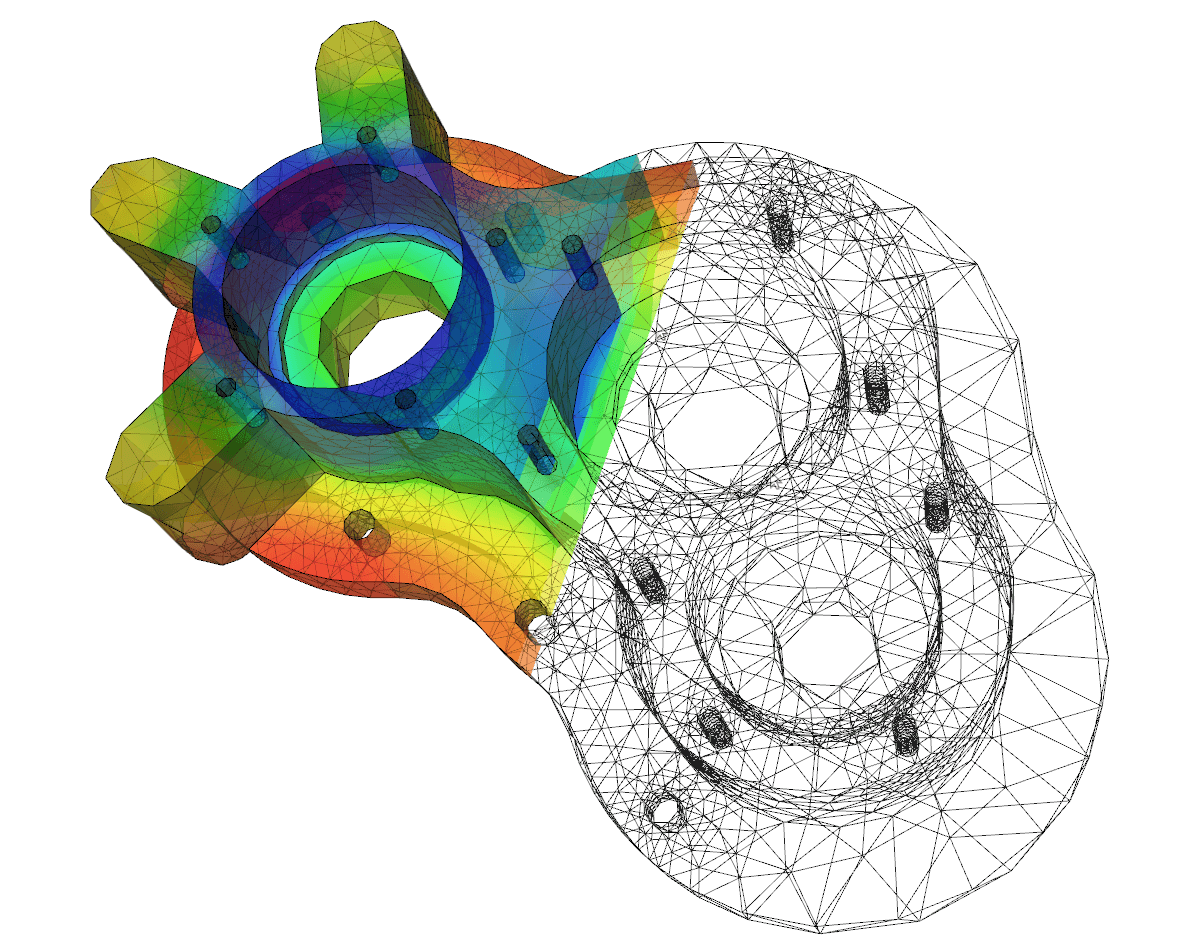
\includegraphics[width=5cm]{../images/elmer-pump-heatequation.png}};
    \end{tikzpicture}
  }

  \begin{frame}{Where do we stand?}
    \begin{center}
      \begin{tabular}{|c|l|l|l|}
        \hline
        \rowcolor{darkred!20}\textbf{Week} & \textbf{Module}                          & \textbf{Lecture topic}           & \textbf{Mini-projects} \\
        \hline
        1                                  & \multirow{3}{7em}{Linear elastodynamics} & Strong and weak forms            &                        \\ \cline{1-1} \cline{3-4}
        2                                  &                                          & Galerkin and FE methods          &                        \\ \cline{1-1} \cline{3-4}
        3                                  &                                          & Systematisation of the procedure & Groups formation       \\ \cline{1-1} \cline{3-4}
        \hline
      \end{tabular}
    \end{center}
    \vspace{1cm}
  \end{frame}

  \begin{frame}
    \textbf{\large Summary}
    \begin{itemize}
      \item Recap week 2
      \item FEM in global coordinate system
            \begin{itemize}
              \item 1D and 2D elements and shape functions
              \item Example: longitudinal vibration of a bar
            \end{itemize}
      \item FEM in local coordinate system
            \begin{itemize}
              \item Localization and elementary quantities
              \item Automating integration and archetypal shape functions
              \item Example: dynamic analysis of a clamped beam
            \end{itemize}
    \end{itemize}
    \vspace{.5cm}

    \textbf{\large Recommended readings}
    \begin{enumerate}
      \item Gmür, Dynamique des structures (§3.1, §3.2 and §3.3)
      \item Neto et al., Engineering Computation of Structures (§2.3 and Chapter 7)
    \end{enumerate}
  \end{frame}


  \section{Recap week 2 \\ Discretisation with Galerkin method}
   {\setbeamercolor{background canvas}{bg=darkred!5}
    \setbeamercolor{block body}{bg=darkred!5,fg=black}

    \begin{frame}{Formulations of elastodynamics}
      \vspace{-0.35cm}
      \begin{columns}[T,onlytextwidth]
        % Left: spatial domain and displacement field
        \begin{column}{0.3\textwidth}
          \centering
          \textbf{Undeformed solid}
          \vspace{0.5cm}
          \newline
          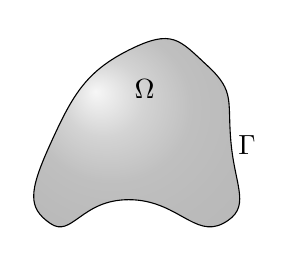
\begin{tikzpicture}
            % Draw the potato-like shape
            \shade [ball color= gray!50!black, opacity=.3] plot [thick,smooth cycle, tension=1] coordinates  {(1,2) (2,3.2) (3,3) (3.3,2) (3.2,1) (2,1.3) (1,1)};
            \draw plot [thick,smooth cycle, tension=1] coordinates {(1,2) (2,3.2) (3,3) (3.3,2) (3.2,1) (2,1.3) (1,1)};
            % Label the region Omega	
            \node at (2.2,2.7) {$\Omega$};
            % Label the boundary Gamma
            \node at (3.5,2) {$\Gamma$};
          \end{tikzpicture}
          \textbf{Deformed solid}
          \vspace{0.5cm}
          \newline
          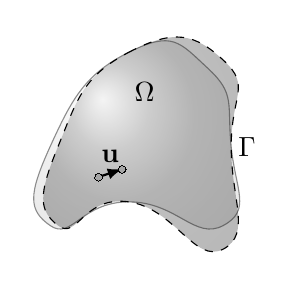
\begin{tikzpicture}
            % Draw the potato-like shape
            \shade [ball color= gray!90, opacity=.1] plot [thick,smooth cycle, tension=1] coordinates  {(1,2) (2,3.2) (3,3) (3.3,2) (3.2,1) (2,1.3) (1,1)};
            \draw[color=gray!90] plot [opacity=.1,smooth cycle, tension=1] coordinates {(1,2) (2,3.2) (3,3) (3.3,2) (3.2,1) (2,1.3) (1,1)};
            \shade [ball color= gray!50!black, opacity=.3] plot [thick,smooth cycle, tension=1] coordinates  {(1.1,2) (2,3.2) (3.2,3.1) (3.3,2) (3.2,0.7) (2,1.3) (1.1,1)};
            \draw[dashed] plot [color=gray!40!black, opacity=.3,thick, smooth cycle, tension=1] coordinates {(1.1,2) (2,3.2) (3.2,3.1) (3.3,2) (3.2,0.7) (2,1.3) (1.1,1)};
            % Label the region Omega	
            \node at (2.2,2.7) {$\Omega$};
            % Label the boundary Gamma
            \node at (3.5,2) {$\Gamma$};
            \draw[thick,-latex] (2,2,1) to node[midway,above]{$\mathbf u$} (2.3,2.1,1);
            \node[draw,shape=circle,fill=black!35,minimum size=1mm,line width=0mm,inner sep=0] at (2,2,1) {};
            \node[draw,shape=circle,fill=black!35,minimum size=1mm,line width=0mm,inner sep=0] at (2.3,2.1,1) {};
          \end{tikzpicture}
        \end{column}

        % Right: formulation sequence
        \begin{column}{0.65\textwidth}
          \centering
          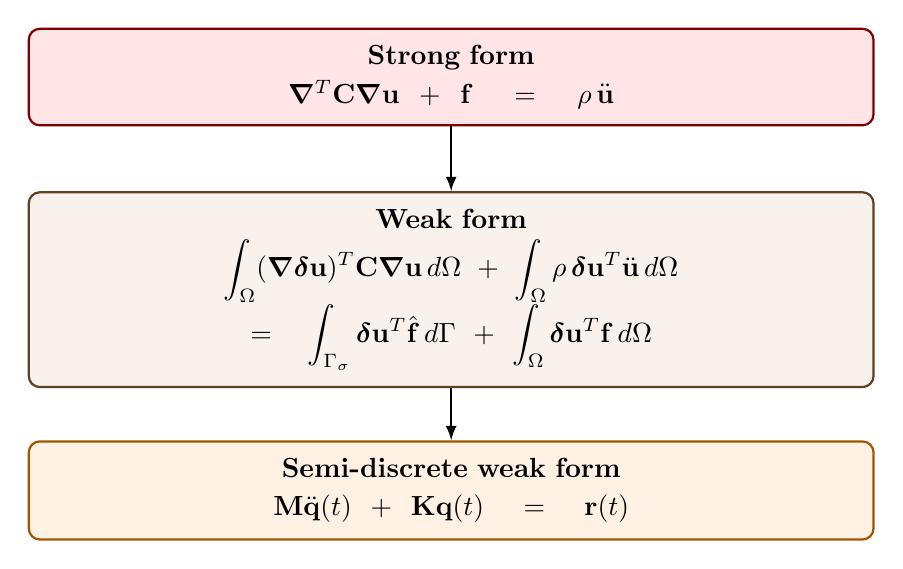
\begin{tikzpicture}[
              box/.style={draw,rounded corners,thick,align=center,inner sep=6pt,
                  text width=.85\linewidth},
              flow/.style={-latex,thick}
            ]
            \node[box,draw=red!50!black,fill=red!10] (sf) at (0,0) {
              \textbf{Strong form}\\[2pt]
              $\boldsymbol{\nabla}^{T}\mathbf C\boldsymbol{\nabla}\mathbf u
                +\mathbf f=\rho\,\ddot{\mathbf u}$
            };
            \node[box,draw=brown!50!black,fill=brown!10] (wf) at (0,-2.7) {
              \textbf{Weak form}\\[3pt]
              $\displaystyle
                \int_{\Omega}(\boldsymbol{\nabla}\bolddelta\mathbf u)^T
                \mathbf C\boldsymbol{\nabla}\mathbf u\,d\Omega
                +\int_{\Omega}\rho\,\bolddelta\mathbf u^T\ddot{\mathbf u}\,d\Omega$
              \\
              $\displaystyle
                =\int_{\Gamma_{\sigma}}\bolddelta\mathbf u^T\hat{\mathbf f}\,d\Gamma
                +\int_{\Omega}\bolddelta\mathbf u^T\mathbf f\,d\Omega$
            };
            \node[box,draw=orange!65!black,fill=orange!10] (sdwf) at (0,-5.25) {
              \textbf{Semi-discrete weak form}\\[2pt]
              $\mathbf M\ddot{\mathbf q}(t)+\mathbf K\mathbf q(t)=\mathbf r(t)$
            };
            \draw[flow] (sf.south) -- (wf.north);
            \draw[flow] (wf.south) -- (sdwf.north);
          \end{tikzpicture}
        \end{column}
      \end{columns}
    \end{frame}

    \begin{frame}{Galerkin method}
      \begin{center}
        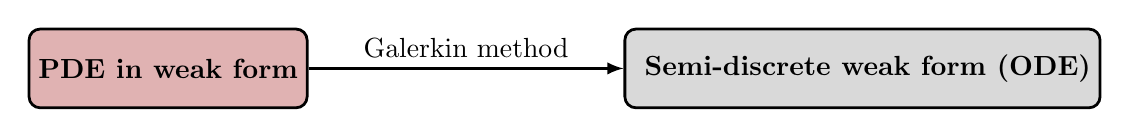
\begin{tikzpicture}
          % Draw first rectangle with PDE label
          \node[draw, rounded corners, minimum width=2cm, minimum height=1cm, fill=darkred!30,line width=1pt] (PDE) {\textbf{PDE in weak form}};

          % Draw second rectangle with ODE label
          \node[draw, rounded corners, minimum width=2cm, minimum height=1cm, right=4cm of PDE, fill=gray!30,line width=1pt] (ODE) {\textbf{ Semi-discrete weak form (ODE)}};

          % Draw arrow with Galerkin method label
          \draw[-latex,line width=1pt] (PDE) -- (ODE) node[midway, above] {Galerkin method};
        \end{tikzpicture}
      \end{center}
      \textbf{Shape functions:} $$\mathbf u^{h}(\mathbf x,t)=\mathbf H(\mathbf x)\mathbf q(t)\qquad\text{and}\qquad \bolddelta\mathbf u^{h}(\mathbf x)=\mathbf H(\mathbf x)\bolddelta\mathbf q.$$
      \vspace{-0.9cm}
      {\footnotesize
        \begin{block}{}
          $$
            \begin{pmatrix}
              u_{1}^{h}(\mathbf x,t) \\
              u_{2}^{h}(\mathbf x,t) \\
              u_{3}^{h}(\mathbf x,t) \\
            \end{pmatrix}
            =
            \begin{bmatrix}
              h_{11}(\mathbf x) & h_{12}(\mathbf x) & \dots & h_{1n}(\mathbf x) \\
              h_{21}(\mathbf x) & h_{22}(\mathbf x) & \dots & h_{2n}(\mathbf x) \\
              h_{31}(\mathbf x) & h_{32}(\mathbf x) & \dots & h_{3n}(\mathbf x) \\
            \end{bmatrix}
            \begin{pmatrix}
              q_{1}(t) \\
              q_{2}(t) \\
              \vdots   \\
              q_{n}(t)
            \end{pmatrix}
          $$

          $$
            \begin{pmatrix}
              \delta u_{1}^{h}(\mathbf x) \\
              \delta u_{2}^{h}(\mathbf x) \\
              \delta u_{3}^{h}(\mathbf x) \\
            \end{pmatrix}
            =
            \begin{bmatrix}
              h_{11}(\mathbf x) & h_{12}(\mathbf x) & \dots & h_{1n}(\mathbf x) \\
              h_{21}(\mathbf x) & h_{22}(\mathbf x) & \dots & h_{2n}(\mathbf x) \\
              h_{31}(\mathbf x) & h_{32}(\mathbf x) & \dots & h_{3n}(\mathbf x) \\
            \end{bmatrix}
            \begin{pmatrix}
              \delta  q_{1} \\
              \delta q_{2}  \\
              \vdots        \\
              \delta  q_{n}
            \end{pmatrix}
          $$
        \end{block}
      }
    \end{frame}

    \begin{frame}{Definitions}
      \begin{columns}[onlytextwidth]
        \begin{column}{0.68\textwidth}
          \begin{block}{}
            \begin{itemize}
              \item \textbf{Stiffness matrix} ($n\times n$):
                    \[
                      \mathbf K
                      = \int_\Omega \mathbf B^T \mathbf C \mathbf B\,d\Omega
                    \]
                    $\mathbf B$ is the ($6\times n$) deformation matrix : $\mathbf B=\boldsymbol{\nabla}\mathbf H$.

              \item \textbf{Mass matrix} ($n\times n$):
                    \[
                      \mathbf M
                      = \int_\Omega \rho\,\mathbf H^T\mathbf H\,d\Omega.
                    \]

              \item \textbf{Applied forces vector} ($n\times 1$):
                    \[
                      \mathbf r(t)
                      = \int_{\Gamma_\sigma}\mathbf H^T\mathbf{\hat f}\,d\Gamma
                      + \int_\Omega\mathbf H^T\mathbf f\,d\Omega.
                    \]
            \end{itemize}
          \end{block}
        \end{column}

        \begin{column}{0.29\textwidth}
          \begin{tcolorbox}[colback=darkred!10,colframe=darkred!40!black,]
            \vspace{-0.5cm}
            \[
              \boldsymbol{\nabla} =
              \begin{bmatrix}
                \partial_x & 0          & 0          \\
                0          & \partial_y & 0          \\
                0          & 0          & \partial_z \\
                0          & \partial_z & \partial_y \\
                \partial_z & 0          & \partial_x \\
                \partial_y & \partial_x & 0
              \end{bmatrix}
            \]
          \end{tcolorbox}
        \end{column}
      \end{columns}
    \end{frame}

    \begin{frame}{Advantages and drawbacks of Galerkin method}
      \begin{columns}
        \begin{column}{0.5\textwidth}
          \textbf{Advantages:}
          \begin{itemize}
            \item[\Checkmark]Converges quickly with appropriate shape functions.
            \item[\Checkmark]  Provides a systematic and structured approach for approximating solutions.
            \item[\Checkmark] The same set of functions is used to express real and virtual variables.
          \end{itemize}
        \end{column}

        \begin{column}{0.5\textwidth}
          \textbf{Drawbacks:}
          \begin{itemize}
            \item[\XSolidBrush] Accuracy heavily dependent on choice of basis functions.
            \item[\XSolidBrush]No physical interpretation of the unknown variable $\mathbf q(t)$.
            \item[\XSolidBrush] The formulation of initial and boundary conditions in the discretized form is cumbersome.
          \end{itemize}
        \end{column}
      \end{columns}
    \end{frame}

    \begin{frame}{Displacements approximation in finte element method}
      \vspace{-1cm}
      \begin{columns}[T]
        \begin{column}{.4\textwidth}
          \begin{center}
            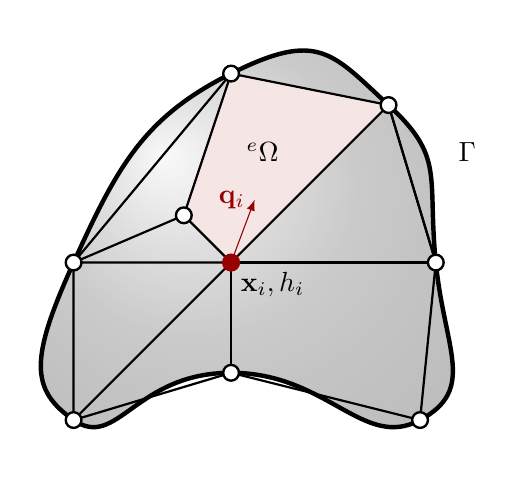
\begin{tikzpicture}[scale=2]
              %\draw[step=1.0,black,thin] (0,0) grid (4,4);
              % Draw the potato-like shape
              \shade [ball color= gray!90!black, opacity=.3] plot [thick,smooth cycle, tension=1] coordinates  {(1,2) (2,3.2) (3,3) (3.3,2) (3.2,1) (2,1.3) (1,1)};
              \draw[ultra thick] plot [thick,smooth cycle, tension=1] coordinates {(1,2) (2,3.2) (3,3) (3.3,2) (3.2,1) (2,1.3) (1,1)};
              \draw[fill=darkred!30,thick,darkred!10] (2,2) -- (3,3) -- (2,3.2) -- (1.7,2.3) -- cycle;
              \node[below right] at (2,2) {$\mathbf x_i, h_i$};
              \draw[-latex,darkred] (2,2) -- (2.15,2.4) node[darkred, left]{$\mathbf q_i$};
              % Label the region Omega	
              \node at (2.2,2.7) {${}^e\Omega$};
              % Label the boundary Gamma
              \node at (3.5,2.7) {$\Gamma$};
              \draw[thick] (1,2) -- (2,3.2) -- (3,3) -- (3.3,2) -- (3.2,1) -- (2,1.3) -- (1,1) -- cycle;
              \draw[thick] (1,2) -- (2,2) -- (3,3) -- (3.3,2);
              \draw[thick] (2,1.3) -- (2,2) -- (3.3,2);
              \draw[thick] (1,1) -- (2,2) -- (1.7,2.3) -- (2,3.2);
              \draw[thick] (1.7,2.3) -- (1,2);
              \node[darkred,draw,shape=circle,fill=darkred,minimum size=2mm,line width=0.3mm,inner sep=0] at (2,2) {};
              \node[draw,shape=circle,fill=white,minimum size=2mm,line width=0.3mm,inner sep=0] at (1,1) {};
              \node[draw,shape=circle,fill=white,minimum size=2mm,line width=0.3mm,inner sep=0] at (1,2) {};
              \node[draw,shape=circle,fill=white,minimum size=2mm,line width=0.3mm,inner sep=0] at (2,1.3) {};
              \node[draw,shape=circle,fill=white,minimum size=2mm,line width=0.3mm,inner sep=0] at (2,3.2) {};
              \node[draw,shape=circle,fill=white,minimum size=2mm,line width=0.3mm,inner sep=0] at (1.7,2.3) {};
              \node[draw,shape=circle,fill=white,minimum size=2mm,line width=0.3mm,inner sep=0] at (3,3) {};
              \node[draw,shape=circle,fill=white,minimum size=2mm,line width=0.3mm,inner sep=0] at (3.2,1) {};
              \node[draw,shape=circle,fill=white,minimum size=2mm,line width=0.3mm,inner sep=0] at (3.3,2) {};
            \end{tikzpicture}
          \end{center}
        \end{column}
        \begin{column}{.6\textwidth}
          Let $p$ the number of nodes of the mesh.
          \vspace{-.2cm}
          \begin{align*}
            \mathbf u^{h}(\mathbf x,t) & =\mathbf H(\mathbf x)\mathbf q(t) = \sum_{i=1}^{p}h_{i}(\mathbf x)\mathbf q_{i}(t)
          \end{align*}
          \vspace{-.5cm}
          \begin{itemize}
            \item $\mathbf H(\mathbf x)$ is a $3\times 3p$ matrix of \textbf{shape functions}:
                  $$
                    \mathbf H
                    =\left[
                      \begin{array}{c;{2pt/2pt}c;{2pt/2pt}c;{2pt/2pt}c;{2pt/2pt}c;{2pt/2pt}c}
                        h_{1}\mathbf I & h_{2}\mathbf I & \dots & h_{i}\mathbf I & \dots & h_{p}\mathbf I \\
                      \end{array} \right]
                  $$
                  $\mathbf I$ is the $3\times 3$ identity matrix.
            \item $\mathbf q(t)$ is a $3p\times 1$ vector of (\emph{unknown}) \textbf{nodal displacements}.

          \end{itemize}
        \end{column}
      \end{columns}
    \end{frame}


    \begin{frame}{Global nodal shape functions requirements}
      \vspace{-1cm}
      \begin{columns}[T]
        \begin{column}{.4\textwidth}
          \begin{center}
            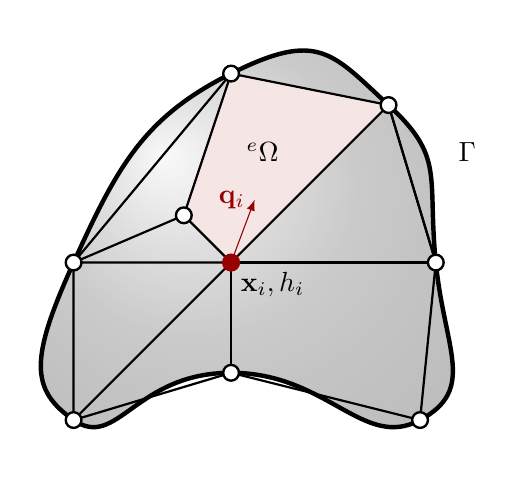
\begin{tikzpicture}[scale=2]
              %\draw[step=1.0,black,thin] (0,0) grid (4,4);
              % Draw the potato-like shape
              \shade [ball color= gray!90!black, opacity=.3] plot [thick,smooth cycle, tension=1] coordinates  {(1,2) (2,3.2) (3,3) (3.3,2) (3.2,1) (2,1.3) (1,1)};
              \draw[ultra thick] plot [thick,smooth cycle, tension=1] coordinates {(1,2) (2,3.2) (3,3) (3.3,2) (3.2,1) (2,1.3) (1,1)};
              \draw[fill=darkred!30,thick,darkred!10] (2,2) -- (3,3) -- (2,3.2) -- (1.7,2.3) -- cycle;
              \node[below right] at (2,2) {$\mathbf x_i, h_i$};
              \draw[-latex,darkred] (2,2) -- (2.15,2.4) node[darkred, left]{$\mathbf q_i$};
              % Label the region Omega	
              \node at (2.2,2.7) {${}^e\Omega$};
              % Label the boundary Gamma
              \node at (3.5,2.7) {$\Gamma$};
              \draw[thick] (1,2) -- (2,3.2) -- (3,3) -- (3.3,2) -- (3.2,1) -- (2,1.3) -- (1,1) -- cycle;
              \draw[thick] (1,2) -- (2,2) -- (3,3) -- (3.3,2);
              \draw[thick] (2,1.3) -- (2,2) -- (3.3,2);
              \draw[thick] (1,1) -- (2,2) -- (1.7,2.3) -- (2,3.2);
              \draw[thick] (1.7,2.3) -- (1,2);
              \node[darkred,draw,shape=circle,fill=darkred,minimum size=2mm,line width=0.3mm,inner sep=0] at (2,2) {};
              \node[draw,shape=circle,fill=white,minimum size=2mm,line width=0.3mm,inner sep=0] at (1,1) {};
              \node[draw,shape=circle,fill=white,minimum size=2mm,line width=0.3mm,inner sep=0] at (1,2) {};
              \node[draw,shape=circle,fill=white,minimum size=2mm,line width=0.3mm,inner sep=0] at (2,1.3) {};
              \node[draw,shape=circle,fill=white,minimum size=2mm,line width=0.3mm,inner sep=0] at (2,3.2) {};
              \node[draw,shape=circle,fill=white,minimum size=2mm,line width=0.3mm,inner sep=0] at (1.7,2.3) {};
              \node[draw,shape=circle,fill=white,minimum size=2mm,line width=0.3mm,inner sep=0] at (3,3) {};
              \node[draw,shape=circle,fill=white,minimum size=2mm,line width=0.3mm,inner sep=0] at (3.2,1) {};
              \node[draw,shape=circle,fill=white,minimum size=2mm,line width=0.3mm,inner sep=0] at (3.3,2) {};
            \end{tikzpicture}
          \end{center}
        \end{column}
        \begin{column}{.6\textwidth}
          \textbf{Propretries of $h_i$:}
          \begin{itemize}
            \item Linearly independent polynomial basis.
            \item Satisfy Kronecker delta property:
                  $$ h_i(\mathbf{x}_i) = 1\quad\text{and} \quad h_i(\mathbf{x}_j) = 0.$$
            \item Vanish on non-adjacent elements.
            \item Continuous at interfaces.
            \item Differentiable inside elements.
            \item Ensure rigid body motion \& constant deformations.\vspace{-0.1cm}
                  $$\sum_{i=1}^{p}h_{i}(\mathbf x)=1 \quad\text{and}\quad \sum_{i=1}^{p}\boldsymbol\nabla h_{i}(\mathbf x)=\mathbf 0.$$
          \end{itemize}
        \end{column}
      \end{columns}
    \end{frame}

    \begin{frame}{Types of analysis}
      \begin{columns}[T,onlytextwidth]
        % ============================================================
        % STATIC
        % ============================================================
        \begin{column}{0.31\textwidth}
          \begin{block}{Static analysis}
            \centering
            \small
            \emph{Constant loads}

            \vspace{0.25cm}

            Determines the structural deformation
            $\mathbf q$ due to constant loads.
          \end{block}
        \end{column}

        % ============================================================
        % MODAL
        % ============================================================
        \begin{column}{0.31\textwidth}
          \begin{block}{Modal analysis}
            \centering
            \small
            \emph{Natural frequencies}

            \vspace{0.25cm}

            Studies the intrinsic dynamic properties of the structure.
          \end{block}
        \end{column}

        % ============================================================
        % TRANSIENT
        % ============================================================
        \begin{column}{0.31\textwidth}

          \begin{block}{Transient analysis}
            \centering
            \small
            \emph{Time-dependent loads}

            \vspace{0.25cm}

            Determines the structural response
            $\mathbf q(t)$ to time-dependent excitations
            $\mathbf r(t)$.
          \end{block}
        \end{column}
      \end{columns}

      \vspace{-0.5cm}

      \begin{columns}[T,onlytextwidth]
        % ============================================================
        % STATIC
        % ============================================================
        \begin{column}{0.31\textwidth}
          \begin{block}{}
            \centering
            \small
            \[
              \mathbf K\mathbf q=\mathbf r
            \]
            \vspace{-0.45cm}
            \footnotesize
            \begin{itemize}
              \item No inertia effects
              \item No time dependence
              \item Equilibrium between internal and external forces
            \end{itemize}
          \end{block}
        \end{column}

        % ============================================================
        % MODAL
        % ============================================================
        \begin{column}{0.31\textwidth}
          \begin{block}{}
            \centering
            \small
            \[
              \mathbf M\ddot{\mathbf q}(t)
              +
              \mathbf K\mathbf q(t)
              =
              \mathbf 0
            \]
            \vspace{-0.45cm}
            \footnotesize
            \begin{itemize}
              \item No external excitation
              \item Resonance when excitation frequency $\approx$ natural frequency
            \end{itemize}
          \end{block}
        \end{column}

        % ============================================================
        % TRANSIENT
        % ============================================================
        \begin{column}{0.31\textwidth}

          \begin{block}{}
            \centering
            \small
            \[
              \mathbf M\ddot{\mathbf q}(t)
              +
              \mathbf K\mathbf q(t)
              =
              \mathbf r(t)
            \]
            \vspace{-0.45cm}
            \footnotesize
            \begin{itemize}
              \item Inertia effects included
              \item Response evolves in time
              \item Used for impacts, vibrations and dynamic loading
            \end{itemize}
          \end{block}
        \end{column}
      \end{columns}
    \end{frame}

    \begin{frame}{Modal analysis}
      \vspace{-0.2cm}
      \begin{itemize}
        \item Free vibrations: $\mathbf f=0$, thus $\mathbf r(t)=\mathbf 0$.
        \item Assume harmonic solution: $$\mathbf q(t)=\mathbf p \alpha \cos (\omega t-\varphi)$$
              \vspace{-0.6cm}
              \begin{itemize}
                \item $\mathbf p$ is the mode shape (eigenvector).
                \item $\omega$ is the natural angular frequency (eigenvalue) [rad/s].
                \item Regular frequency $f=\omega/2\pi$ [Hz].
                \item $\alpha$ (amplitude) and $\varphi$ (phase) depend on initial conditions.
              \end{itemize}
        \item Leads to the eigenvalue problem:
              $$(\mathbf K-\omega^2\mathbf M)\mathbf p=\mathbf 0.$$
        \item Non-trivial solutions exist only if:
              $$\det(\mathbf K-\omega^2\mathbf M)=0.$$
              The eigenvalues $\lambda_i=\omega_i^2$ are the squares of the natural angular frequencies. \newline
              The eigenvectors $\mathbf p_i$ are the corresponding mode shapes.
      \end{itemize}
    \end{frame}
   }

  \section{1D and 2D elements and global shape functions}

  \begin{frame}{Shape functions for one dimensional structures}
    \begin{center}
      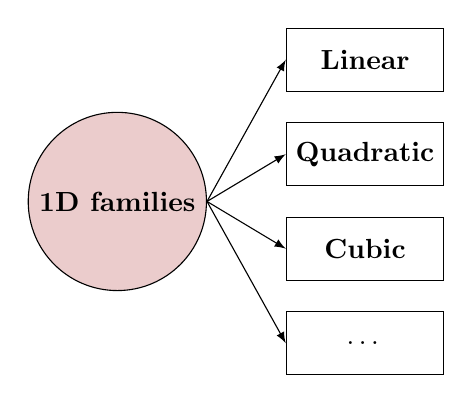
\begin{tikzpicture}
        % Draw the main circle labeled "1D"
        \node[circle, draw, minimum size=1.5cm, fill=darkred!20] (circle) at (0,0) {\textbf{1D families}};
        % Define the list of polynomial degrees
        \foreach \i/\txt in {1/Linear, 2/Quadratic, 3/Cubic, 4/$\dots$} {
            % Compute y-shift to center the list
            \pgfmathsetmacro{\yshift}{(2.5-\i) * 1.2}

            % Draw rectangles with text
            \node[draw, minimum width=2cm, minimum height=0.8cm, right=1cm of circle, yshift=\yshift cm] (box\i) {\textbf{\txt}};

            % Draw connecting arrows
            \draw[-latex] (circle.east) -- (box\i.west);
          }
      \end{tikzpicture}
    \end{center}
  \end{frame}

  \begin{frame}{1D finite elements}
    \begin{center}
      \begin{figure}
        \begin{subfigure}{0.45\textwidth}
          \centering
          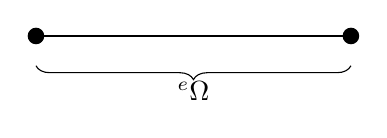
\begin{tikzpicture}
            % Define points
            \coordinate (A) at (-2, 0);
            \coordinate (B) at (2, 0);
            % Mark points
            \fill (A) circle (3pt);
            \fill (B) circle (3pt);
            % Label the element
            \draw[thick] (A) --(B);
            \draw [decorate,decoration={brace,amplitude=5pt,mirror,raise=2.5ex}]
            (A) -- (B) node[midway,yshift=-2em]{${}^{e}\Omega$};
          \end{tikzpicture}
          \caption{Linear element}
          \label{fig:subfig1}
        \end{subfigure}
        \hfill
        \begin{subfigure}{0.45\textwidth}
          \centering
          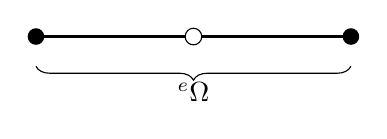
\begin{tikzpicture}
            % Define points
            \coordinate (A) at (-2, 0);
            \coordinate (B) at (2, 0);
            \coordinate (C) at (0, 0);
            \draw[thick] (A) --(B);
            % Mark points
            \fill (A) circle (3pt);
            \fill (B) circle (3pt);
            \draw[fill=white, draw=black] (C) circle (3pt);
            % Label the element
            \draw [decorate,decoration={brace,amplitude=5pt,mirror,raise=2.5ex}]
            (A) -- (B) node[midway,yshift=-2em]{${}^{e}\Omega$};
          \end{tikzpicture}
          \caption{Quadratic element}
          \label{fig:subfig2}
        \end{subfigure}

        \vspace{1cm}

        \begin{subfigure}{0.45\textwidth}
          \centering
          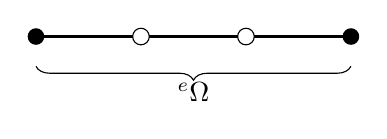
\begin{tikzpicture}
            % Define points
            \coordinate (A) at (-2, 0);
            \coordinate (B) at (2, 0);
            \coordinate (C) at (-2/3, 0);
            \coordinate (D) at (2/3, 0);
            \draw[thick] (A) --(B);
            % Mark points
            \fill (A) circle (3pt);
            \fill (B) circle (3pt);
            \draw[fill=white, draw=black] (C) circle (3pt);
            \draw[fill=white, draw=black](D) circle (3pt);
            % Label the element
            \draw [decorate,decoration={brace,amplitude=5pt,mirror,raise=2.5ex}]
            (A) -- (B) node[midway,yshift=-2em]{${}^{e}\Omega$};
          \end{tikzpicture}
          \caption{Cubic element}
          \label{fig:subfig3}
        \end{subfigure}
        \hfill
        \begin{subfigure}{0.45\textwidth}
          \centering
          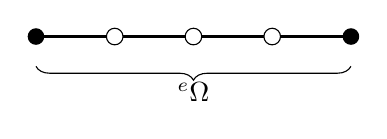
\begin{tikzpicture}
            % Define points
            \coordinate (A) at (-2, 0);
            \coordinate (B) at (2, 0);
            \coordinate (C) at (-1, 0);
            \coordinate (D) at (0, 0);
            \coordinate (E) at (1, 0);
            \draw[thick] (A) --(B);
            % Mark points
            \fill (A) circle (3pt);
            \fill (B) circle (3pt);
            \draw[fill=white, draw=black] (C) circle (3pt);
            \draw[fill=white, draw=black] (D) circle (3pt);
            \draw[fill=white, draw=black] (E) circle (3pt);
            % Label the element
            \draw [decorate,decoration={brace,amplitude=5pt,mirror,raise=2.5ex}]
            (A) -- (B) node[midway,yshift=-2em]{${}^{e}\Omega$};
          \end{tikzpicture}
          \caption{Quartic element}
          \label{fig:subfig4}
        \end{subfigure}
      \end{figure}
    \end{center}
  \end{frame}

  \begin{frame}{Linear shape functions}
    \begin{columns}
      \begin{column}{.5\textwidth}
        \begin{center}
          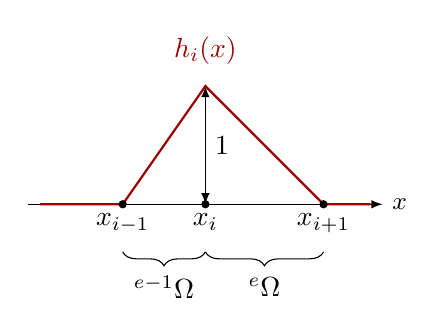
\begin{tikzpicture}[scale=1.5]
            % Draw axes
            \draw[-latex] (-1.5, 0) -- (1.5, 0) node[right] {\small $x$};
            \draw[latex-latex] (0, 0) -- (0, 1) node[right, midway] {$1$};
            % Define points
            \coordinate (A) at (-0.7, 0);
            \coordinate (B) at (0, 1);
            \coordinate (O) at (0, 0);
            \coordinate (C) at (1, 0);
            % Draw the linear shape function
            \draw[thick, darkred] (-1.4, 0) -- (A) -- (B) -- (C) -- (1.4, 0);
            % Mark points
            \fill (A) circle (1pt) node[below] {$x_{i-1}$};
            \fill (O) circle (1pt) node[below] {$x_i$};
            \fill (C) circle (1pt) node[below] {$x_{i+1}$};
            % Label the function
            \node[darkred, above] at (0, 1.1) {$h_i(x)$};
            \draw [decorate,decoration={brace,amplitude=5pt,mirror,raise=4ex}]
            (A) -- (O) node[midway,yshift=-3em]{${}^{e-1}\Omega$};
            \draw [decorate,decoration={brace,amplitude=5pt,mirror,raise=4ex}]
            (O) -- (C) node[midway,yshift=-3em]{${}^{e}\Omega$};
          \end{tikzpicture}
        \end{center}
      \end{column}
      \begin{column}{.6\textwidth}
        {\small $$h_i(x) =
            \begin{cases}
              l_2[x_{i-1},x_i](x)=\dfrac{x - x_{i-1}}{x_i - x_{i-1}} & x\in{}^{e-1}\Omega \\[10pt]
              l_1[x_{i},x_{i+1}](x)= \dfrac{x-x_{i+1}}{x_i-x_{i+1}}  & x\in{}^{e}\Omega   \\[10pt]
              0                                                      & \text{otherwise}
            \end{cases} $$}
      \end{column}
    \end{columns}
    {\small \begin{itemize}
      \item \( h_i \) are piecewise linear functions that, within each finite element, corresponds to a first-degree Lagrange polynomial:
            $$l_j[x_1,\dots,x_n](x)=\prod_{\substack{m=1 \\ m\neq j}}^{n}\frac{x-x_m}{x_j-x_m}$$
      \item Any linear piecewise function can be expressed as a linear combination of the \( h_i \).
    \end{itemize}}
  \end{frame}

  \begin{frame}{1D displacement approximation via linear shape functions}
    $$u^{h}(x,t)=\sum_{i=1}^{p}h_{i}(x)q_{i}(t)$$
    \begin{center}
      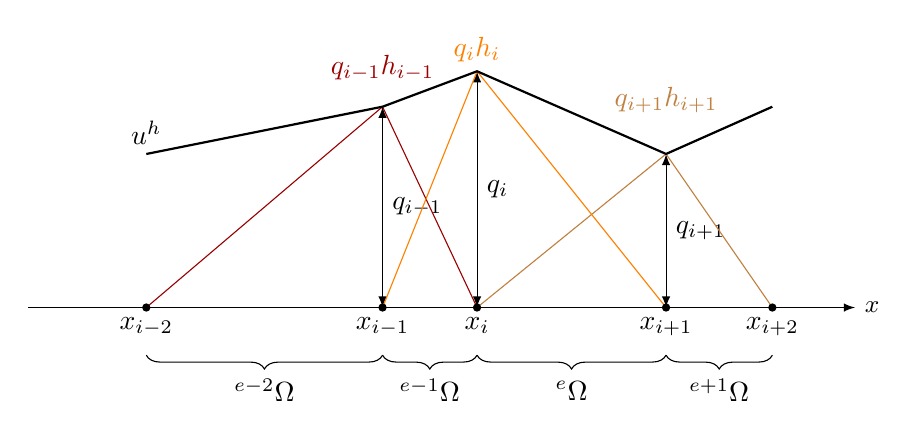
\begin{tikzpicture}[scale=1.5]
        % Draw axes
        \draw[-latex] (-3, 0) -- (4, 0) node[right] {\small $x$};
        % Define points
        \coordinate (A) at (-2, 0);
        \coordinate (H) at (0, 1.7);
        \coordinate (O) at (0, 0);
        \coordinate (B) at (0.8, 0);
        \coordinate (C) at (2.4, 0);
        \coordinate (D) at (3.3, 0);
        \coordinate (J) at (2.4, 1.3);
        \coordinate (K) at (0.8, 2);
        % Draw the linear shape function
        \draw[latex-latex,thin] (O) -- (H) node[right, midway] {$q_{i-1}$};
        \draw[latex-latex,thin] (B) -- (K) node[right, midway] {$q_{i}$};
        \draw[latex-latex,thin] (C) -- (J) node[right, midway] {$q_{i+1}$};
        \draw[darkred] (A) -- (H) -- (B);
        \draw[brown]  (B) -- (J) -- (D) ;
        \draw[orange]  (O) -- (K) -- (C) ;
        \draw[thick]  (-2,1.3) -- (H) -- (K) -- (J) -- (3.3,1.7);
        % Mark points
        \fill (A) circle (1pt) node[below] {$x_{i-2}$};
        \fill (O) circle (1pt) node[below] {$x_{i-1}$};
        \fill (B) circle (1pt) node[below] {$x_{i}$};
        \fill (C) circle (1pt) node[below] {$x_{i+1}$};
        \fill (D) circle (1pt) node[below] {$x_{i+2}$};
        % Label the function
        \node[darkred, above=0.2cm] at (H) {$q_{i-1}h_{i-1}$};
        \node[brown, above=0.4cm] at (J) {$q_{i+1}h_{i+1}$};
        \node[orange, above] at (K) {$q_{i}h_{i}$};
        \node[above] at (-2,1.3) {$u^h$};
        \draw [decorate,decoration={brace,amplitude=5pt,mirror,raise=4ex}]
        (A) -- (O) node[midway,yshift=-3em]{${}^{e-2}\Omega$};
        \draw [decorate,decoration={brace,amplitude=5pt,mirror,raise=4ex}]
        (O) -- (B) node[midway,yshift=-3em]{${}^{e-1}\Omega$};
        \draw [decorate,decoration={brace,amplitude=5pt,mirror,raise=4ex}]
        (B) -- (C) node[midway,yshift=-3em]{${}^{e}\Omega$};
        \draw [decorate,decoration={brace,amplitude=5pt,mirror,raise=4ex}]
        (C) -- (D) node[midway,yshift=-3em]{${}^{e+1}\Omega$};
      \end{tikzpicture}
    \end{center}
  \end{frame}

  \begin{frame}{Quadratic shape functions}
    \begin{columns}
      \begin{column}{.5\textwidth}
        \hspace{.1cm} If $i$ is even:
        \vspace{-0.7cm}
        \begin{center}
          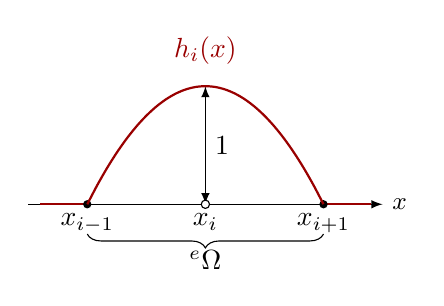
\begin{tikzpicture}[scale=1.5]
            % Draw axes
            \draw[-latex] (-1.5, 0) -- (1.5, 0) node[right] {\small $x$};
            \draw[latex-latex] (0, 0) -- (0, 1) node[right, midway] {$1$};
            % Define points
            \coordinate (A) at (-1, 0);
            \coordinate (B) at (0, 1);
            \coordinate (O) at (0, 0);
            \coordinate (C) at (1, 0);
            % Draw the linear shape function
            \draw[thick, darkred] (-1.4, 0) -- (A);
            \draw[thick, darkred] (C) -- (1.4, 0);
            % Mark points
            \fill (A) circle (1pt) node[below] {$x_{i-1}$};
            \draw[fill=white, draw=black] (O) circle (1pt) node[below] {$x_{i}$};
            \fill (C) circle (1pt) node[below] {$x_{i+1}$};
            % Label the function
            \draw[thick, darkred, domain=-1:1, smooth, variable=\x] plot ({\x}, {-\x*\x +1});
            \node[darkred, above] at (0, 1.1) {$h_i(x)$};
            \draw [decorate,decoration={brace,amplitude=5pt,mirror,raise=2.5ex}]
            (A) -- (C) node[midway,yshift=-2em]{${}^{e}\Omega$};
          \end{tikzpicture}
        \end{center}
      \end{column}
      \begin{column}{.6\textwidth}
        {\small $$h_i(x) =
            \begin{cases}
              l_2[x_{i-1},x_i,x_{i+1}](x) & x\in{}^{e}\Omega \\[10pt]
              0                           & \text{otherwise}
            \end{cases} $$}
      \end{column}
    \end{columns}
    \vspace{0.5cm}
    \begin{columns}
      \begin{column}{.6\textwidth}
        If $i$ is odd:
        \vspace{-0.65cm}
        \begin{center}
          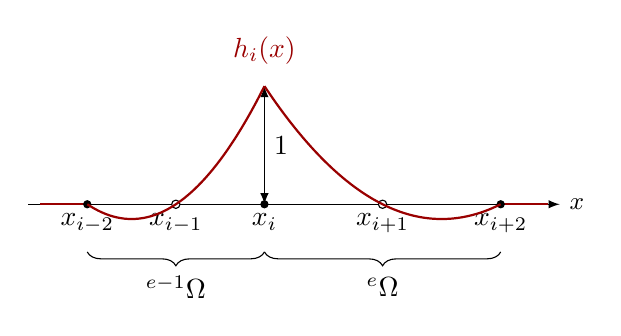
\begin{tikzpicture}[scale=1.5]
            % Draw axes
            \draw[-latex] (-2, 0) -- (2.5, 0) node[right] {\small $x$};
            \draw[latex-latex] (0, 0) -- (0, 1) node[right, midway] {$1$};
            % Define points
            \coordinate (A) at (-1.5, 0);
            \coordinate (B) at (-0.75, 0);
            \coordinate (O) at (0, 0);
            \coordinate (H) at (1, 0);
            \coordinate (C) at (1, 0);
            \coordinate (D) at (2, 0);
            % Draw the linear shape function
            \draw[thick, darkred] (-1.9, 0) -- (A);
            \draw[thick, darkred] (D) -- (2.4, 0);
            % Mark points
            \fill (A) circle (1pt) node[below] {$x_{i-2}$};
            \fill (O) circle (1pt) node[below] {$x_{i}$};
            \fill (D) circle (1pt) node[below] {$x_{i+2}$};
            \draw[fill=white, draw=black] (B) circle (1pt) node[below] {$x_{i-1}$};
            \draw[fill=white, draw=black] (C) circle (1pt) node[below] {$x_{i+1}$};
            % Label the function
            \draw[thick, darkred,domain=-1.5:0, smooth, variable=\x]
            plot ({\x}, {((\x + 1.5) * (\x + 0.75)) / 1.125});
            \draw[thick, darkred,domain=0:2, smooth, variable=\x]
            plot ({\x}, {((\x - 1) * (\x - 2)) / 2}) ;
            \node[darkred, above] at (0, 1.1) {$h_i(x)$};
            \draw [decorate,decoration={brace,amplitude=5pt,mirror,raise=4ex}]
            (A) -- (O) node[midway,yshift=-3em]{${}^{e-1}\Omega$};
            \draw [decorate,decoration={brace,amplitude=5pt,mirror,raise=4ex}]
            (O) -- (D) node[midway,yshift=-3em]{${}^{e}\Omega$};
          \end{tikzpicture}
        \end{center}
      \end{column}
      \begin{column}{.45\textwidth}
        {\small $$h_i(x) =
            \begin{cases}
              l_3[x_{i-2},x_{i-1},x_{i}](x) & x\in{}^{e-1}\Omega \\[10pt]
              l_1[x_{i},x_{i+1},x_{i+2}](x) & x\in{}^{e}\Omega   \\[10pt]
              0                             & \text{otherwise}
            \end{cases} $$}
      \end{column}
    \end{columns}
  \end{frame}

  \begin{frame}{Examples of 1D displacement approximation}
    \begin{center}
      \begin{figure}
        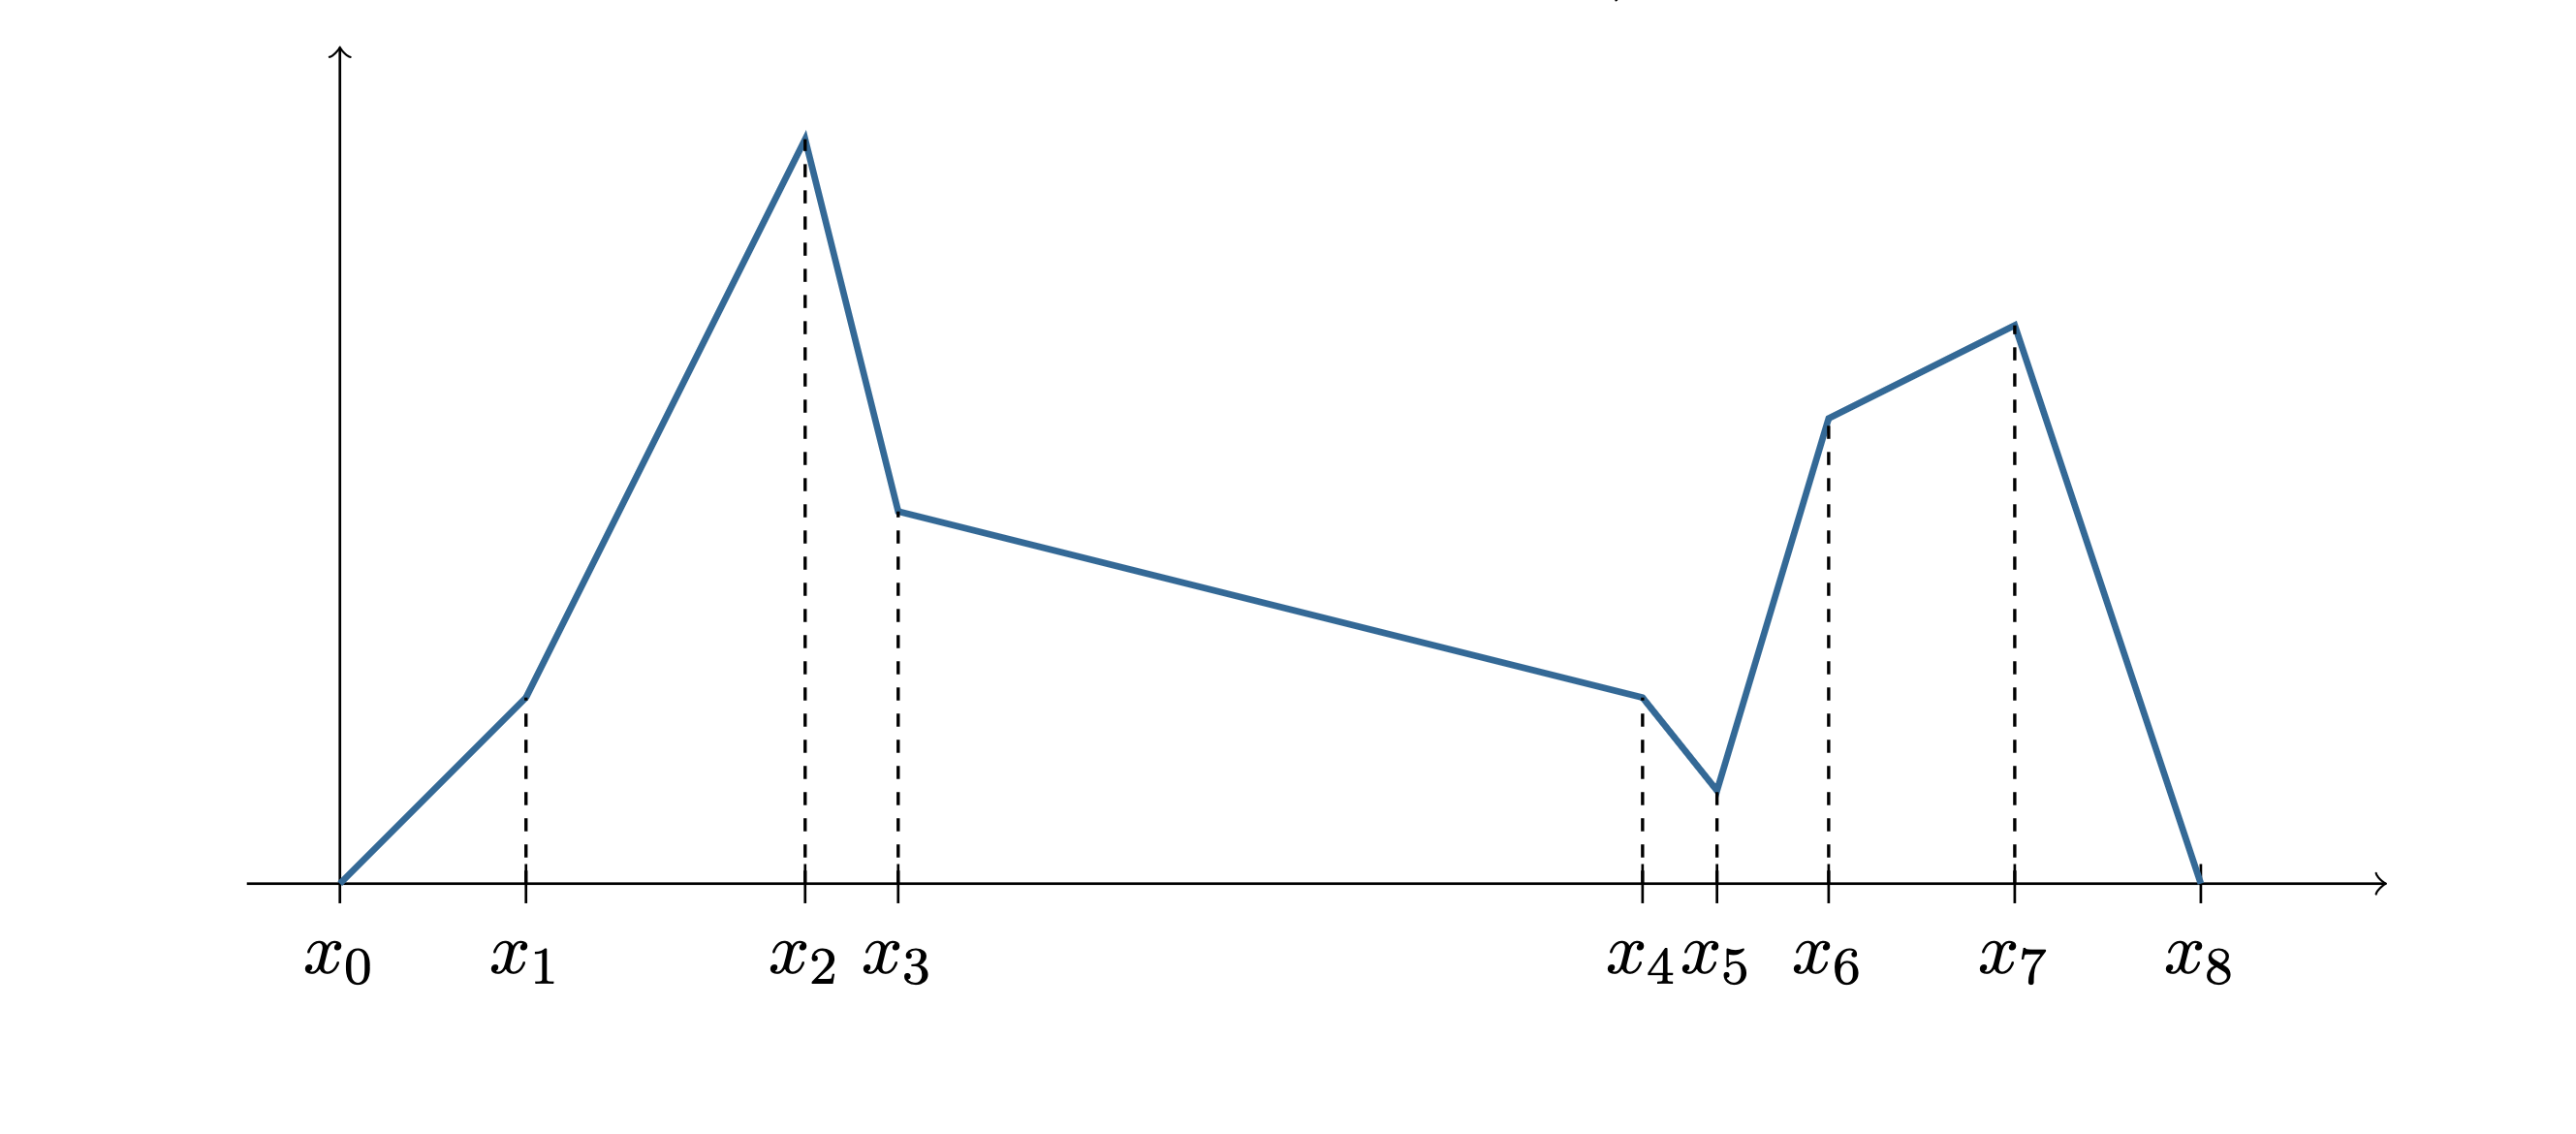
\includegraphics[width=0.45\textwidth]{../images/dispApproxLin.png}
        \caption*{Displacement approximation via linear shape functions}
        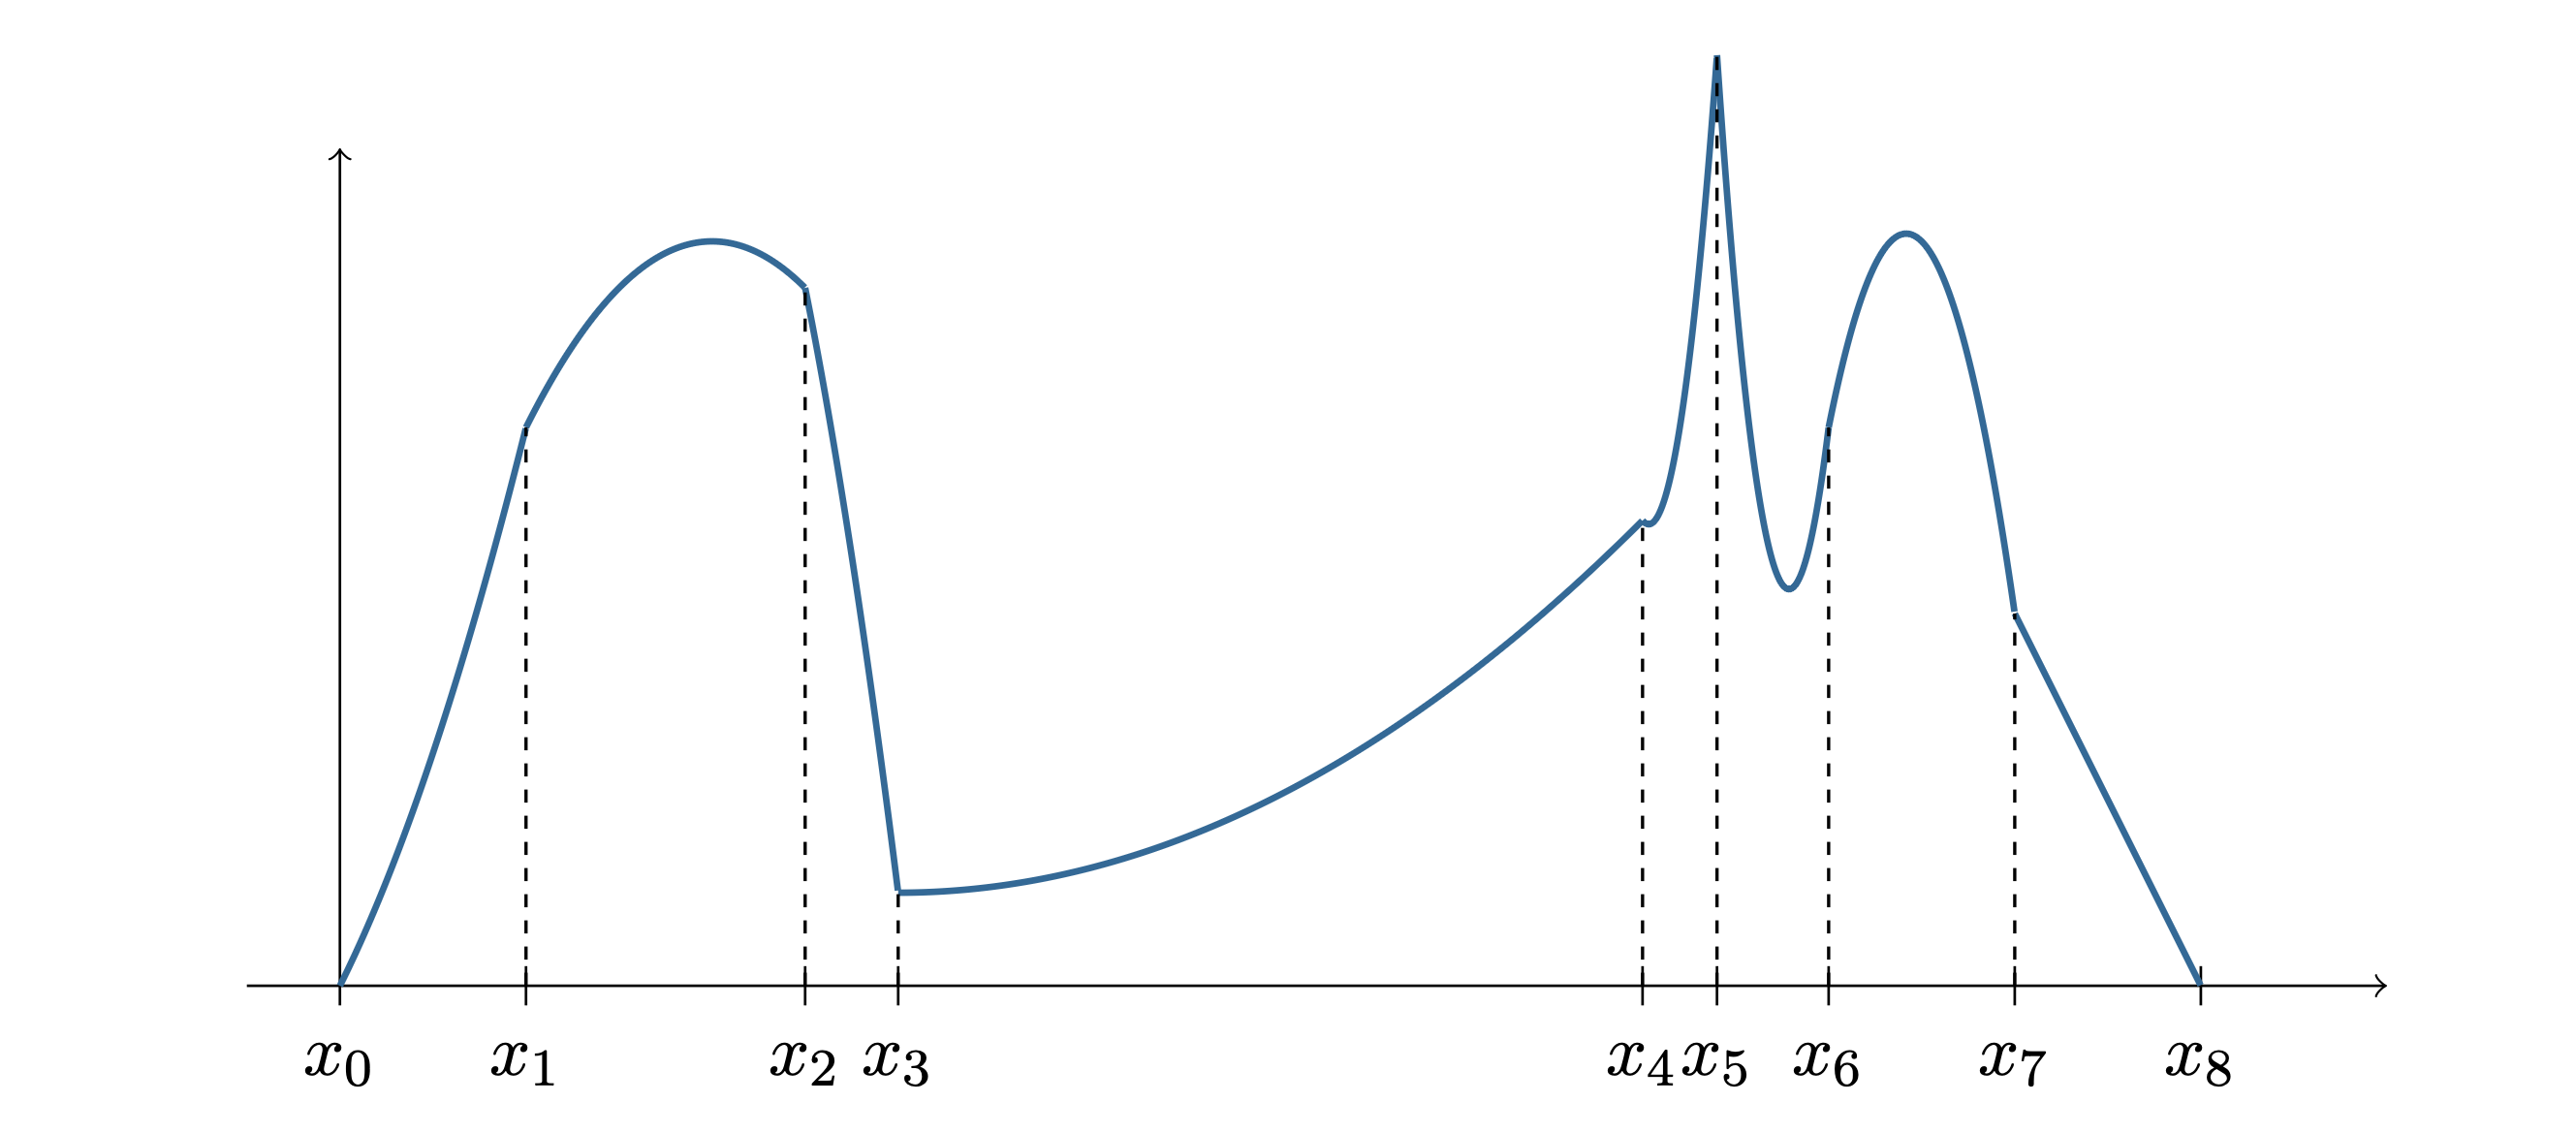
\includegraphics[width=0.45\textwidth]{../images/dispApproxQuad.png}
        \caption*{Displacement approximation via quadratic shape functions}
      \end{figure}
    \end{center}
  \end{frame}

  \begin{frame}{Shape functions for two-dimensional structures}
    \begin{center}
      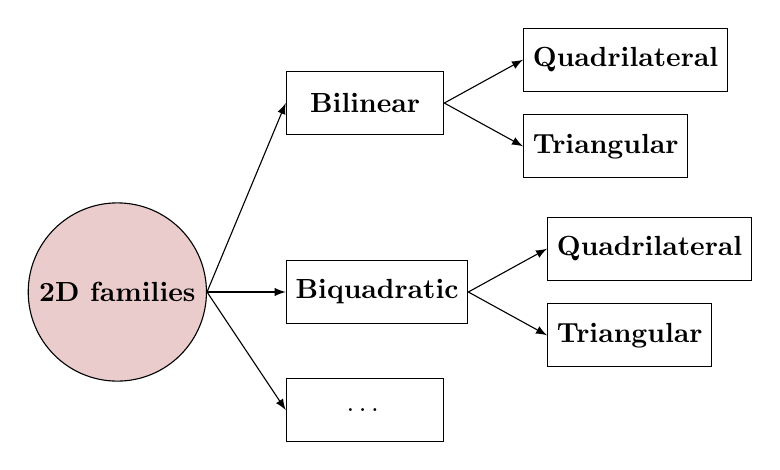
\begin{tikzpicture}
        % Draw the main circle labeled "2D"
        \node[circle, draw, minimum size=1cm, fill=darkred!20] (circle) at (0,0) {\textbf{2D families}};
        % Define the list of polynomial degrees
        \foreach \i/\txt in {1/Bilinear, 2/Biquadratic} {
            % Compute y-shift to center the list
            \pgfmathsetmacro{\yshift}{(2-\i) * 2.4}
            % Draw rectangles with text
            \node[draw, minimum width=2cm, minimum height=0.8cm, right=1cm of circle, yshift=\yshift cm] (box\i) {\textbf{\txt}};
            % Draw connecting arrows
            \draw[-latex] (circle.east) -- (box\i.west);
            \foreach \j/\txt in {1/Quadrilateral, 2/Triangular} {
                % Compute y-shift to center the list
                \pgfmathsetmacro{\ysecondShift}{(1.5-\j) * 1.1}
                % Draw rectangles with text
                \node[draw, minimum width=2cm, minimum height=0.8cm, right=1cm of box\i, yshift=\ysecondShift cm] (secondBox\j) {\textbf{\txt}};
                % Draw connecting arrows
                \draw[-latex] (box\i.east) -- (secondBox\j.west);
              }
          }
        \node[draw, minimum width=2cm, minimum height=0.8cm, right=1cm of circle, yshift=-1.5 cm] (box) {$\dots$};
        % Draw connecting arrows
        \draw[-latex] (circle.east) -- (box.west);
      \end{tikzpicture}
    \end{center}
  \end{frame}


  \begin{frame}{2D finite elements}
    \begin{center}
      \begin{figure}
        \begin{subfigure}{0.45\textwidth}
          \centering
          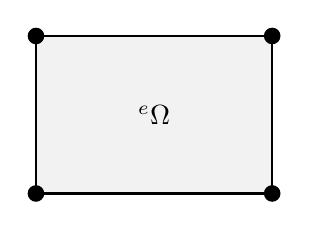
\begin{tikzpicture}
            \def\a{3}
            \def\b{2}
            \coordinate (x1) at (0, 0);
            \coordinate (x2) at (\a, 0);
            \coordinate (x3) at (0, \b);
            \coordinate (x4) at (\a, \b);
            \filldraw[gray!10] (x1) -- (x2) -- (x4) -- (x3) -- cycle;
            \draw[thick] (x1) -- (x2) -- (x4) -- (x3) -- cycle;
            \fill (x1) circle (3pt);
            \fill (x2) circle (3pt);
            \fill (x3) circle (3pt);
            \fill (x4) circle (3pt);
            \node at (\a/2,\b/2) {${}^e\Omega$};
          \end{tikzpicture}
          \caption{Bilinear Quadrilateral}
        \end{subfigure}
        \hfill
        \begin{subfigure}{0.45\textwidth}
          \centering
          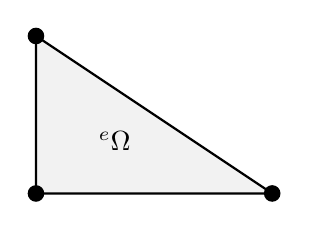
\begin{tikzpicture}
            \def\a{3}
            \def\b{2}
            \coordinate (x1) at (0, 0);
            \coordinate (x2) at (\a, 0);
            \coordinate (x3) at (0, \b);
            \filldraw[gray!10] (x1) -- (x2) -- (x3) -- cycle;
            \draw[thick] (x1) -- (x2)-- (x3) -- cycle;
            \fill (x1) circle (3pt);
            \fill (x2) circle (3pt);
            \fill (x3) circle (3pt);
            \node at (\a/3,\b/3) {${}^e\Omega$};
          \end{tikzpicture}
          \caption{Bilinear Triangular}
        \end{subfigure}

        \vspace{0.5cm}

        \begin{subfigure}{0.45\textwidth}
          \centering
          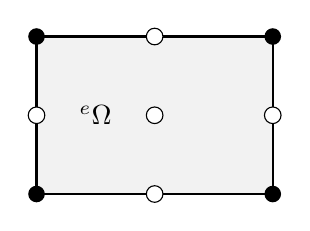
\begin{tikzpicture}
            \def\a{3}
            \def\b{2}
            \coordinate (x1) at (0, 0);
            \coordinate (x2) at (\a/2, 0);
            \coordinate (x3) at (\a, 0);
            \coordinate (x4) at (0, \b/2);
            \coordinate (x5) at (\a/2, \b/2);
            \coordinate (x6) at (\a, \b/2);
            \coordinate (x7) at (0, \b);
            \coordinate (x8) at (\a/2, \b);
            \coordinate (x9) at (\a, \b);
            \filldraw[gray!10] (x1) -- (x3) -- (x9) -- (x7) -- cycle;
            \draw[thick] (x1) -- (x3) -- (x9) -- (x7) -- cycle;
            \fill (x1) circle (3pt);
            \draw[fill=white, draw=black] (x2) circle (3pt);
            \fill (x3) circle (3pt);
            \draw[fill=white, draw=black]  (x4) circle (3pt);
            \draw[fill=white, draw=black] (x5) circle (3pt);
            \draw[fill=white, draw=black] (x6) circle (3pt);
            \fill (x7) circle (3pt);
            \draw[fill=white, draw=black] (x8) circle (3pt);
            \fill (x9) circle (3pt);
            \node at (\a/4,\b/2) {${}^e\Omega$};
          \end{tikzpicture}
          \caption{Biquadratic Quadrilateral}
        \end{subfigure}
        \hfill
        \begin{subfigure}{0.45\textwidth}
          \centering
          \begin{tikzpicture}
            \begin{tikzpicture}
              \def\a{3}
              \def\b{2}
              \coordinate (x1) at (0, 0);
              \coordinate (x2) at (\a, 0);
              \coordinate (x3) at (0, \b);
              \coordinate (x4) at (\a/2,0);
              \coordinate (x5) at (0, \b/2);
              \coordinate (x6) at (\a/2, \b/2);
              \filldraw[gray!10] (x1) -- (x2) -- (x3) -- cycle;
              \draw[thick] (x1) -- (x2)-- (x3) -- cycle;
              \fill (x1) circle (3pt);
              \fill (x2) circle (3pt);
              \fill (x3) circle (3pt);
              \draw[fill=white, draw=black]  (x4) circle (3pt);
              \draw[fill=white, draw=black] (x5) circle (3pt);
              \draw[fill=white, draw=black] (x6) circle (3pt);
              \node at (\a/3,\b/3) {${}^e\Omega$};
            \end{tikzpicture}
          \end{tikzpicture}
          \caption{Biquadratic Triangular}
        \end{subfigure}
      \end{figure}
    \end{center}
  \end{frame}

  \begin{frame}{Bilinear quadrilateral finite elements mesh}
    \begin{center}
      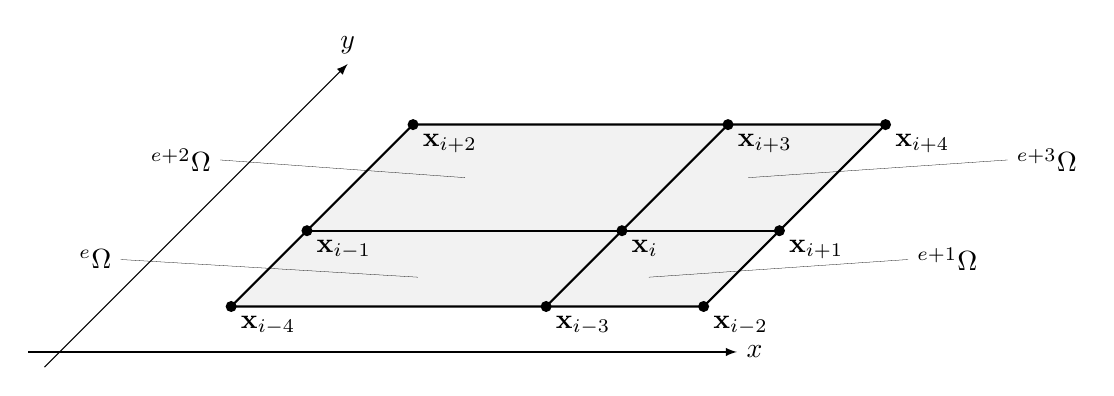
\begin{tikzpicture}
        \def\a{4}
        \def\b{3.5}
        \def\c{6}
        \def\h{1},
        \coordinate (x1) at (0,0, 0);
        \coordinate (x2) at (\a,0, 0);
        \coordinate (x3) at (\c,0, 0);
        \coordinate (x4) at (0,0, \b);
        \coordinate (x5) at (\a,0, \b);
        \coordinate (x51) at (\a,\h, \b);
        \coordinate (x6) at (\c,0, \b);
        \coordinate (x7) at (0,0, \c);
        \coordinate (x8) at (\a,0, \c);
        \coordinate (x9) at (\c,0, \c);
        %Color fill
        \filldraw[gray!10] (x1) -- (x2) -- (x51) -- (x4) -- cycle;
        \filldraw[gray!10] (x2) -- (x51) -- (x6) -- (x3) -- cycle;
        \filldraw[gray!10] (x4) -- (x51) -- (x8) -- (x7) -- cycle;
        \filldraw[gray!10] (x51) -- (x6) -- (x9) -- (x8) -- cycle;
        %Draw labels
        \fill (x1) circle (2pt) node[below right] {$\mathbf x_{i+2}$};
        \fill (x2) circle (2pt) node[below right] {$\mathbf x_{i+3}$};
        \fill (x3) circle (2pt) node[below right] {$\mathbf x_{i+4}$};
        \fill (x4) circle (2pt) node[below right] {$\mathbf x_{i-1}$};
        \fill (x5) circle (2pt) node[below right] {$\mathbf x_{i}$};
        \fill (x6) circle (2pt) node[below right] {$\mathbf x_{i+1}$};
        \fill (x7) circle (2pt) node[below right] {$\mathbf x_{i-4}$};
        \fill (x8) circle (2pt) node[below right] {$\mathbf x_{i-3}$};
        \fill (x9) circle (2pt) node[below right] {$\mathbf x_{i-2}$};
        \draw[ultra thin] (\a/3,0,\b/2) -- (-2,0,\b/3) node[left] {${}^{e+2}\Omega$};
        \draw[ultra thin] (\a/2,0,2.6*\b/3+\c/3) -- (-2,0,2.6*\b/3+\c/3-\b/6) node[left] {${}^{e}\Omega$};
        \draw[ultra thin] (2.2*\a/3+\c/3,0,\b/2) -- (\c+2,0,\b/3)node[right] {${}^{e+3}\Omega$};
        \draw[ultra thin] (2.2*\a/3+\c/3,0,2.6*\b/3+\c/3) -- (\c+2,0,2.6*\b/3+\c/3-\b/6)node[right] {${}^{e+1}\Omega$};
        %Draw lines
        \draw[thick] (x1) -- (x3) -- (x9) -- (x7) -- (x1);
        \draw[thick] (x2) -- (x5) -- (x8);
        \draw[thick] (x4) -- (x5) -- (x6);
        \draw[-latex] (-2, 0,7.5) -- (7,0, 7.5) node[right] {$x$};
        \draw[-latex] (-1.6, 0,8) -- (-1.6,0, -2) node[above] {$y$};
      \end{tikzpicture}
    \end{center}
  \end{frame}

  \begin{frame}{Bilinear quadrilateral shape functions}
    \begin{center}
      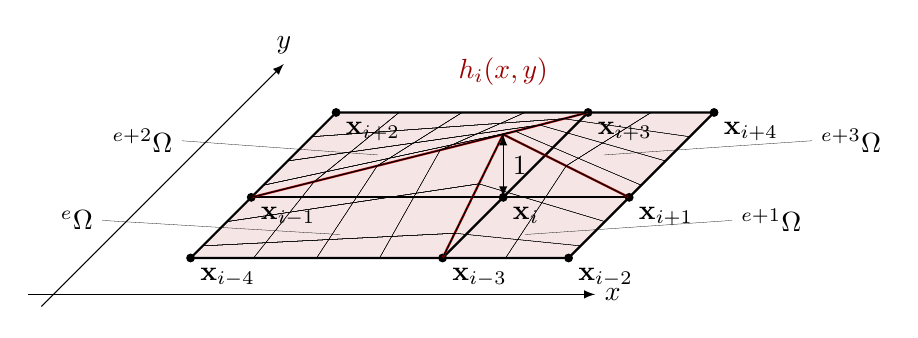
\begin{tikzpicture}[scale=0.8]
        \def\a{4}
        \def\b{3.5}
        \def\c{6}
        \def\h{1},
        \coordinate (x1) at (0,0, 0);
        \coordinate (x2) at (\a,0, 0);
        \coordinate (x3) at (\c,0, 0);
        \coordinate (x4) at (0,0, \b);
        \coordinate (x5) at (\a,0, \b);
        \coordinate (x51) at (\a,\h, \b);
        \coordinate (x6) at (\c,0, \b);
        \coordinate (x7) at (0,0, \c);
        \coordinate (x8) at (\a,0, \c);
        \coordinate (x9) at (\c,0, \c);
        %Color fill
        \filldraw[darkred!10] (x1) -- (x2) -- (x51) -- (x4) -- cycle;
        \filldraw[darkred!10] (x2) -- (x51) -- (x6) -- (x3) -- cycle;
        \filldraw[darkred!10] (x4) -- (x51) -- (x8) -- (x7) -- cycle;
        \filldraw[darkred!10] (x51) -- (x6) -- (x9) -- (x8) -- cycle;
        %Draw labels
        \fill (x1) circle (2pt) node[below right] {$\mathbf x_{i+2}$};
        \fill (x2) circle (2pt) node[below right] {$\mathbf x_{i+3}$};
        \fill (x3) circle (2pt) node[below right] {$\mathbf x_{i+4}$};
        \fill (x4) circle (2pt) node[below right] {$\mathbf x_{i-1}$};
        \fill (x5) circle (2pt) node[below right] {$\mathbf x_{i}$};
        \fill (x6) circle (2pt) node[below right] {$\mathbf x_{i+1}$};
        \fill (x7) circle (2pt) node[below right] {$\mathbf x_{i-4}$};
        \fill (x8) circle (2pt) node[below right] {$\mathbf x_{i-3}$};
        \fill (x9) circle (2pt) node[below right] {$\mathbf x_{i-2}$};
        \draw[ultra thin] (\a/3,0,\b/2) -- (-2,0,\b/3) node[left] {${}^{e+2}\Omega$};
        \draw[ultra thin] (\a/2,0,2.6*\b/3+\c/3) -- (-2,0,2.6*\b/3+\c/3-\b/6) node[left] {${}^{e}\Omega$};
        \draw[ultra thin] (2.2*\a/3+\c/3,0,\b/2) -- (\c+2,0,\b/3)node[right] {${}^{e+3}\Omega$};
        \draw[ultra thin] (2.2*\a/3+\c/3,0,2.6*\b/3+\c/3) -- (\c+2,0,2.6*\b/3+\c/3-\b/6)node[right] {${}^{e+1}\Omega$};
        %Draw lines
        \draw[thick] (x1) -- (x3) -- (x9) -- (x7) -- (x1);
        \draw[thick] (x2) -- (x5) -- (x8);
        \draw[thick] (x4) -- (x5) -- (x6);
        \draw[thick,darkred] (x2) -- (x51);
        \draw[thick,darkred] (x4) -- (x51);
        \draw[thick,darkred] (x6) -- (x51);
        \draw[thick,darkred] (x8) -- (x51);
        \draw[latex-latex] (x5) -- (x51) node[midway,right] {$1$} node[above=0.5cm]{{\color{darkred}$h_i(x,y)$}};
        %draw thin lines
        \foreach \x in {0,...,\a} {
            \foreach \z in {0,...,\b}
              {
                \coordinate (A) at (\x,0,0);
                \coordinate (B) at ($(\x,\h/\a*\x,\b)$);
                \coordinate (C) at (0,0,\z);
                \coordinate (D) at ($(\a,\h/\b*\z,\z)$);
                \draw[ultra thin] (A) -- (B);
                \draw[ultra thin] (C) -- (D);
              }
          }
        \foreach \x in {\a,...,\c} {
            \foreach \z in {0,...,\b}
              {
                \pgfmathsetmacro\dx{\h-\h/(\c-\a)*(\x-\a)}
                \coordinate (A) at (\x,0,0);
                \coordinate (B) at ($(\x,\dx,\b)$);
                \coordinate (C) at (\c,0,\z);
                \coordinate (D) at ($(\a,\h/\b*\z,\z)$);
                \draw[ultra thin] (A) -- (B);
                \draw[ultra thin] (C) -- (D);
              }
          }
        \foreach \x in {0,...,\a} {
            \foreach \z in {\b,...,\c}
              {
                \pgfmathsetmacro\dz{\h-\h/(\c-\b)*(\z-\b)}
                \coordinate (A) at (\x,0,\c);
                \coordinate (B) at ($(\x,\h/\a*\x,\b)$);
                \coordinate (C) at (0,0,\z);
                \coordinate (D) at ($(\a,\dz,\z)$);
                \draw[ultra thin] (A) -- (B);
                \draw[ultra thin] (C) -- (D);
              }
          }
        \foreach \x in {\a,...,\c} {
            \foreach \z in {\b,...,\c}
              {
                \pgfmathsetmacro\dx{\h-\h/(\c-\a)*(\x-\a)}
                \pgfmathsetmacro\dz{\h-\h/(\c-\b)*(\z-\b)}
                \coordinate (A) at (\x,0,\c);
                \coordinate (B) at ($(\x,\dx,\b)$);
                \coordinate (C) at (\c,0,\z);
                \coordinate (D) at ($(\a,\dz,\z)$);
                \draw[ultra thin] (A) -- (B);
                \draw[ultra thin] (C) -- (D);
              }
          }
        \draw[-latex] (-2, 0,7.5) -- (7,0, 7.5) node[right] {$x$};
        \draw[-latex] (-1.6, 0,8) -- (-1.6,0, -2) node[above] {$y$};
      \end{tikzpicture}
    \end{center}
    $$h_i(x,y)=\begin{cases}
        l_2[x_{i-1},x_i](x)l_2[y_{i-3},y_i](y)     & x\in{}^{e}\Omega   \\
        l_1[x_{i},x_{i+1}](x)l_2[y_{i-3},y_{i}](y) & x\in{}^{e+1}\Omega \\
        l_2[x_{i-1},x_{i}](x)l_1[y_{i},y_{i+3}](y) & x\in{}^{e+2}\Omega \\
        l_1[x_{i},x_{i+1}](x)l_1[y_{i},y_{i+3}](y) & x\in{}^{e+3}\Omega \\
        0                                          & \text{otherwise}
      \end{cases}$$
  \end{frame}

  \begin{frame}{Bilinear triangular finite elements mesh}
    \begin{center}
      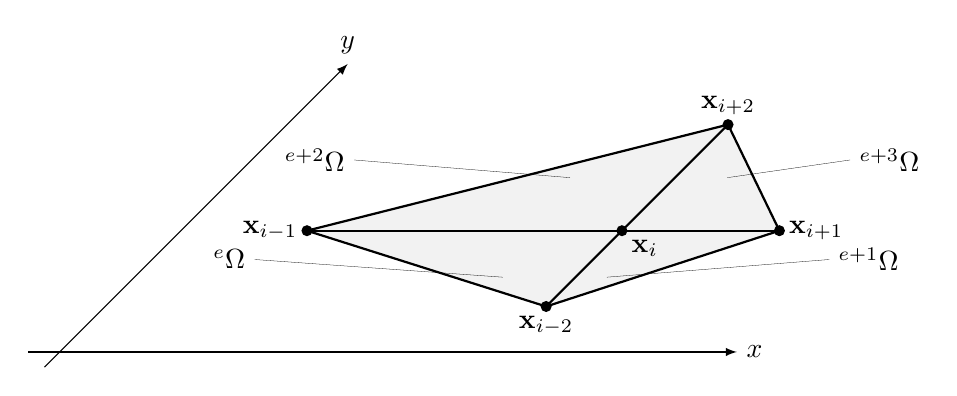
\begin{tikzpicture}
        \def\a{4}
        \def\b{3.5}
        \def\c{6}
        \def\h{1.4},
        \coordinate (x2) at (\a,0, 0);
        \coordinate (x4) at (0,0, \b);
        \coordinate (x5) at (\a,0, \b);
        \coordinate (x51) at (\a,\h, \b);
        \coordinate (x6) at (\c,0, \b);
        \coordinate (x8) at (\a,0, \c);
        %Color fill
        \filldraw[gray!10] (x2) -- (x5) -- (x4) -- cycle;
        \filldraw[gray!10] (x2) -- (x5) -- (x6) -- cycle;
        \filldraw[gray!10] (x4) -- (x5) -- (x8) -- cycle;
        \filldraw[gray!10] (x5) -- (x6) -- (x8) -- cycle;
        %Draw labels
        \fill (x2) circle (2pt) node[above] {$\mathbf x_{i+2}$};
        \fill (x4) circle (2pt) node[left] {$\mathbf x_{i-1}$};
        \fill (x5) circle (2pt) node[below right] {$\mathbf x_{i}$};
        \fill (x6) circle (2pt) node[right] {$\mathbf x_{i+1}$};
        \fill (x8) circle (2pt) node[below] {$\mathbf x_{i-2}$};
        \draw[ultra thin] (\a/1.5,0,\b/2) -- (-0.3,0,\b/3) node[left] {${}^{e+2}\Omega$};
        \draw[ultra thin] (\a/1.3,0,2.6*\b/3+\c/3) -- (-0.3,0,2.6*\b/3+\c/3-\b/6) node[left] {${}^{e}\Omega$};
        \draw[ultra thin] (2*\a/3+\c/3,0,\b/2) -- (\c,0,\b/3)node[right] {${}^{e+3}\Omega$};
        \draw[ultra thin] (1.8*\a/3+\c/3,0,2.6*\b/3+\c/3) -- (\c+1,0,2.6*\b/3+\c/3-\b/6)node[right] {${}^{e+1}\Omega$};
        %Draw lines
        \draw[thick] (x2) -- (x6) -- (x8) -- (x4) -- cycle;
        \draw[thick] (x2) -- (x5) -- (x8);
        \draw[thick] (x4) -- (x5) -- (x6);
        \draw[-latex] (-2, 0,7.5) -- (7,0, 7.5) node[right] {$x$};
        \draw[-latex] (-1.6, 0,8) -- (-1.6,0, -2) node[above] {$y$};
      \end{tikzpicture}
    \end{center}
  \end{frame}


  \begin{frame}{Bilinear triangular shape functions}
    \begin{center}
      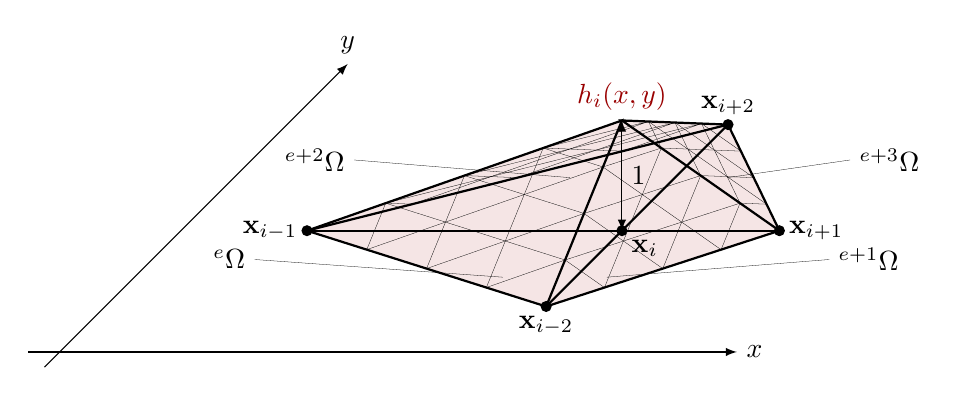
\begin{tikzpicture}
        \def\a{4}
        \def\b{3.5}
        \def\c{6}
        \def\h{1.4},
        \coordinate (x2) at (\a,0, 0);
        \coordinate (x4) at (0,0, \b);
        \coordinate (x5) at (\a,0, \b);
        \coordinate (x51) at (\a,\h, \b);
        \coordinate (x6) at (\c,0, \b);
        \coordinate (x8) at (\a,0, \c);
        %Color fill
        \filldraw[darkred!10] (x2) -- (x51) -- (x4) -- cycle;
        \filldraw[darkred!10] (x2) -- (x51) -- (x6) -- cycle;
        \filldraw[darkred!10] (x4) -- (x51) -- (x8) -- cycle;
        \filldraw[darkred!10] (x51) -- (x6) -- (x8) -- cycle;
        %Draw labels
        \fill (x2) circle (2pt) node[above] {$\mathbf x_{i+2}$};
        \fill (x4) circle (2pt) node[left] {$\mathbf x_{i-1}$};
        \fill (x5) circle (2pt) node[below right] {$\mathbf x_{i}$};
        \fill (x6) circle (2pt) node[right] {$\mathbf x_{i+1}$};
        \fill (x8) circle (2pt) node[below] {$\mathbf x_{i-2}$};
        \draw[ultra thin] (\a/1.5,0,\b/2) -- (-0.3,0,\b/3) node[left] {${}^{e+2}\Omega$};
        \draw[ultra thin] (\a/1.3,0,2.6*\b/3+\c/3) -- (-0.3,0,2.6*\b/3+\c/3-\b/6) node[left] {${}^{e}\Omega$};
        \draw[ultra thin] (2*\a/3+\c/3,0,\b/2) -- (\c,0,\b/3)node[right] {${}^{e+3}\Omega$};
        \draw[ultra thin] (1.8*\a/3+\c/3,0,2.6*\b/3+\c/3) -- (\c+1,0,2.6*\b/3+\c/3-\b/6)node[right] {${}^{e+1}\Omega$};
        %Draw lines
        \draw[thick] (x2) -- (x6) -- (x8) -- (x4) -- cycle;
        \draw[thick] (x2) -- (x5) -- (x8);
        \draw[thick] (x4) -- (x5) -- (x6);
        \draw[latex-latex] (x5) -- (x51) node[midway,right] {$1$} node[above]{{\color{darkred}$h_i(x,y)$}};
        \draw[thick] (x2) -- (x51) -- (x6);
        \draw[thick] (x4) -- (x51) -- (x8);
        %draw thin lines
        \foreach \i in {1,2,3} {
            \pgfmathsetmacro{\t}{\i/4} % Normalize parameter (dividing into 5 segments)
            \pgfmathsetmacro{\x}{(1-\t)*\a} % Linear interpolation for x
            \pgfmathsetmacro{\xb}{\t*\a} % Linear interpolation for x
            \pgfmathsetmacro{\z}{\t*\b}
            \pgfmathsetmacro{\y}{\t*\h} % Linear interpolation for y
            \coordinate (P\i) at (\x, 0, \z);
            \coordinate (Q\i) at (\a, \y, \z);
            \coordinate (R\i) at (\xb, \y, \b);
          }
        \foreach \i in {1, 2, 3} { % Generate 3 equidistant points
            \pgfmathsetmacro{\t}{\i/4} % Normalize the parameter (divide by 4 for 3 points)
            \pgfmathsetmacro{\x}{\t*\a} % Interpolate x-coordinate
            \pgfmathsetmacro{\z}{(1-\t)*\b + \t*\c} % Interpolate z-coordinate
            \coordinate (S\i) at (\x,0, \z); % Define the equidistant point
          }
        \foreach \i in {1, 2, 3} { % Generate 3 equidistant points
            \pgfmathsetmacro{\t}{\i/4} % Normalize the parameter (divide by 4 for 3 points)
            \pgfmathsetmacro{\x}{(1-\t)*\a + \t*\c} % Interpolate x-coordinate
            \pgfmathsetmacro{\z}{(1-\t)*\c + \t*\b} % Interpolate z-coordinate
            \coordinate (T\i) at (\x,0,\z); % Define the equidistant point
          }
        \foreach \i in {1, 2, 3} { % Generate 3 equidistant points
            \pgfmathsetmacro{\t}{\i/4} % Normalize the parameter (divide by 4 for 3 points)
            \pgfmathsetmacro{\x}{(1-\t)*\a + \t*\c} % Interpolate x-coordinate
            \pgfmathsetmacro{\z}{\t*\b} % Interpolate z-coordinate
            \coordinate (U\i) at (\x,0, \z); % Define the equidistant point
          }
        \foreach \i in {1, 2, 3} { % Generate 3 equidistant points
            \pgfmathsetmacro{\t}{\i/4} % Normalize the parameter (divide by 4 for 3 points)
            \pgfmathsetmacro{\x}{(1-\t)*\a + \t*\a} % Interpolate x-coordinate
            \pgfmathsetmacro{\y}{\t*\h} % Interpolate y-coordinate
            \pgfmathsetmacro{\z}{(1-\t)*\c + \t*\b} % Interpolate z-coordinate
            \coordinate (V\i) at (\x, \y, \z); % Define the equidistant point
          }
        \foreach \i in {1, 2, 3} { % Generate 3 equidistant points
            \pgfmathsetmacro{\t}{\i/4} % Normalize the parameter (divide by 4 for 3 points)
            \pgfmathsetmacro{\x}{(1-\t)*\a + \t*\c} % Interpolate x-coordinate
            \pgfmathsetmacro{\y}{(1-\t)*\h } % Interpolate y-coordinate
            \pgfmathsetmacro{\z}{(1-\t)*\b + \t*\b} % Interpolate z-coordinate
            \coordinate (W\i) at (\x, \y, \z); % Define the equidistant point
          }
        \draw[ultra thin] (P3) -- (R1) -- (Q1) -- (P1);
        \draw[ultra thin] (P2) -- (R2) -- (Q2) -- (P2);
        \draw[ultra thin] (P1) -- (R3) -- (Q3) -- (P3);
        \draw[ultra thin] (S1) -- (R1) -- (V1) -- (S3);
        \draw[ultra thin] (S2) -- (R2) -- (V2) -- (S2);
        \draw[ultra thin] (S3) -- (R3) -- (V3) -- (S1);
        \draw[ultra thin] (T1) -- (V1) -- (W3) -- (T3);
        \draw[ultra thin] (T2) -- (V2) -- (W2) -- (T2);
        \draw[ultra thin] (T3) -- (V3) -- (W1) -- (T1);
        \draw[ultra thin] (U1) -- (Q1) -- (W3) -- (U3);
        \draw[ultra thin] (U2) -- (Q2) -- (W2) -- (U2);
        \draw[ultra thin] (U3) -- (Q3) -- (W1) -- (U1);

        %Draw the axis 
        \draw[-latex] (-2, 0,7.5) -- (7,0, 7.5) node[right] {$x$};
        \draw[-latex] (-1.6, 0,8) -- (-1.6,0, -2) node[above] {$y$};
      \end{tikzpicture}
    \end{center}
  \end{frame}

  \section{Example: longitudinal vibration of a bar}

  \begin{frame}{Example - FE approximation of longitudinal vibrations of a bar}
    \begin{columns}
      \column{0.5\textwidth}
      \begin{center}
        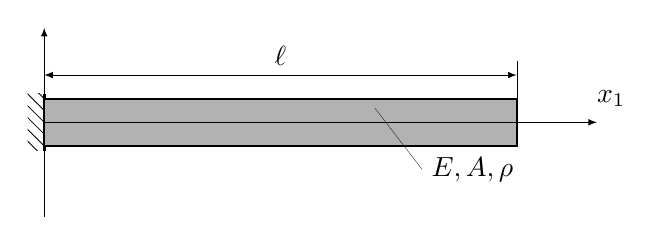
\begin{tikzpicture}[scale=0.6]
          \point{a}{0}{0};
          \support {3}{a}[270];

          % Draw the rectangle
          \filldraw[fill=gray!60, draw=black,thick] (0,-0.5) rectangle (10,0.5);

          %axis
          \draw[-latex, ultra thin] (0,0) -- (11.7,0);
          \draw[-latex, ultra thin] (0,-2) -- (0,2);
          \node at (12,0.5) {\(x_1\)};

          % length
          \draw[ultra thin] (10,0) -- (10, 1.3) ;
          \draw[latex-latex, ultra thin]  (0,1)  to node[sloped,midway,above] {$\ell$}(10,1) ;
          \draw[ultra thin]  (7,0.3) -- (8,-1) node[right]{$E,A,\rho$};
        \end{tikzpicture}
      \end{center}

      \column{0.5\textwidth}
      {\small \begin{itemize}
          \item $A$ cross-sectional area
          \item $\ell$ length
          \item $E$ Young's modulus
          \item $\rho$ material density
          \item $u_1$ axial displacement
          \item $x_1$ axial coordinate
        \end{itemize}}
    \end{columns}

    \vspace{0.3cm}
    \begin{block}{}
      \textbf{Objectives:}
      \begin{enumerate}
        \item Use the finite element method with $n$ linear shape functions to approximate the first two natural frequencies of the bar.
        \item Compare the results with those obtained from Galerkin's approximation.
      \end{enumerate}
    \end{block}
    \begin{center}
      \href{https://drive.mathworks.com/sharing/6a9792ef-d0a7-4aca-a1d0-8b1862b0ac3b}{\beamergotobutton{Go to Matlab Drive}}
    \end{center}
  \end{frame}


  \section{Localization and elementary quantities}

  \begin{frame}{Drawbacks of the global approach}
    \begin{itemize}
      \item[\XSolidBrush] Limited capability in handling complex (unstructured) mesh topologies.
      \item[\XSolidBrush] Computationally expensive: it requires defining one shape function per node.
      \item[\XSolidBrush] Limited utilization of the compact support of nodal shape functions.
    \end{itemize}
    {\color{darkred}\textbf{Local approach:}} provides a quicker and more sistematic way to compute the stiffenss and mass matrices and the applied forces vector:
    \begin{center}
      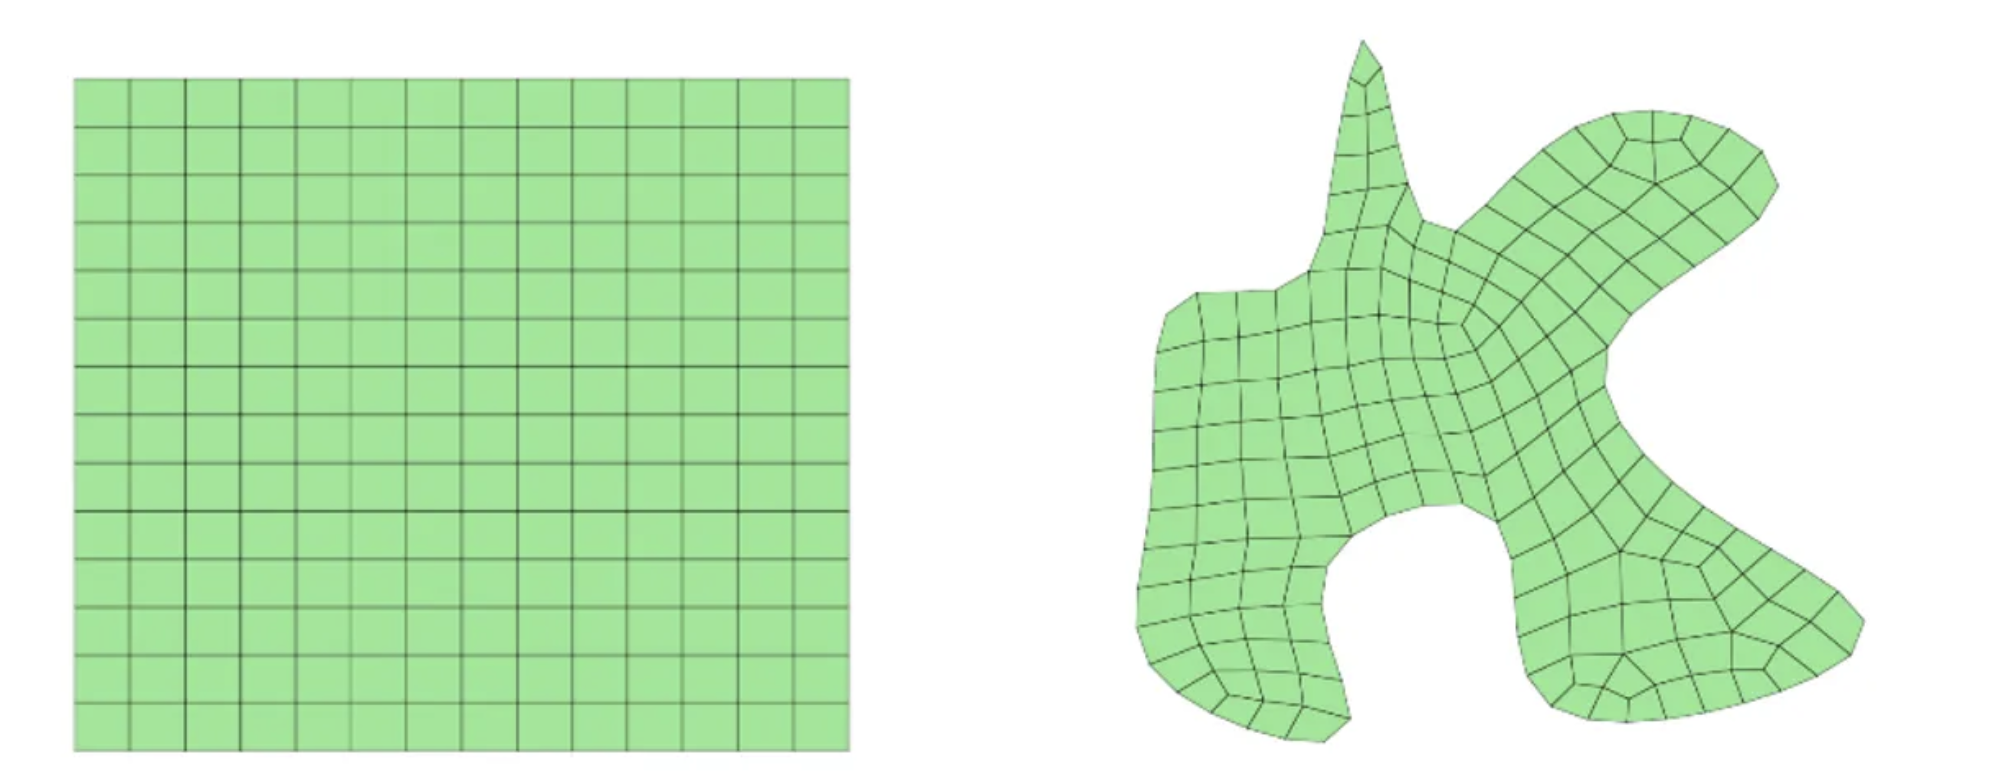
\includegraphics[height=2.5cm]{../images/mesh.png}
    \end{center}
    {\footnotesize (Credit: \hyperlink{https://onscale.com/meshing-in-fea-structured-vs-unstructured-meshes/}{Onscale - structured vs unstructured meshes})}
  \end{frame}
}

\begin{frame}{Localization}
  \begin{columns}[T]
    \begin{column}{.4\textwidth}
      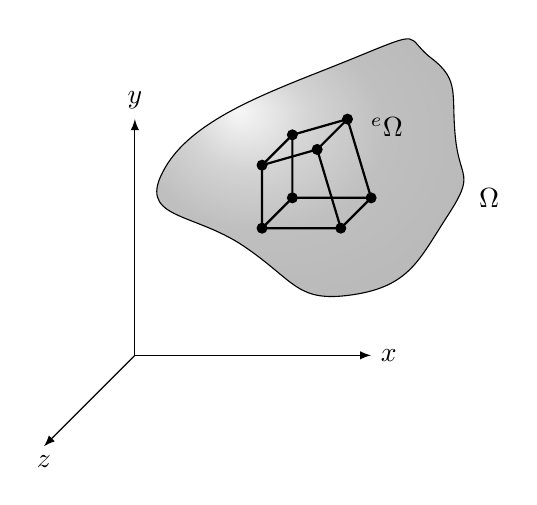
\begin{tikzpicture}
        \draw[-latex] (0,0,0) -- (3,0,0) node[right]{$x$};
        \draw[-latex] (0,0,0) -- (0,3,0) node[above]{$y$};
        \draw[-latex] (0,0,0) -- (0,0,3) node[below]{$z$};
        % Draw the potato-like shape
        \shade [ball color= gray!50!black, opacity=.3] plot [thick,smooth cycle, tension=1] coordinates  {(0,2,-1) (2,3,-2) (3,3,-2) (3.3,2,-2) (3.2,1,-2) (2,0,-2) (1,1,-1)};
        \draw plot [thick,smooth cycle, tension=1] coordinates {(0,2,-1) (2,3,-2) (3,3,-2) (3.3,2,-2) (3.2,1,-2) (2,0,-2) (1,1,-1)};
        % Label the region Omega	
        \node at (3.2,2.9) {${}^e\Omega$};
        % Label the boundary Gamma
        \draw[thick] (2,2,1) -- (2,2.8,1) -- (2.7,3,1) -- (3,2,1) -- cycle;
        \draw[thick] (2,2,0) -- (2,2.8,0) -- (2.7,3,0) -- (3,2,0) -- cycle;
        \draw[thick] (2,2,1) -- (2,2,0);
        \draw[thick] (2,2.8,1) -- (2,2.8,0);
        \draw[thick] (2.7,3,1) -- (2.7,3,0);
        \draw[thick] (3,2,1) -- (3,2,0);
        % Fill vertices
        \foreach \point in {(2,2,1), (2,2.8,1), (2.7,3,1), (3,2,1), (2,2,0), (2,2.8,0), (2.7,3,0), (3,2,0)} {
            \fill \point circle (2pt);
          }
        \node at (4.5,2) {$\Omega$};
      \end{tikzpicture}
    \end{column}
    \hspace{.5cm}
    \begin{column}{.55\textwidth}
      \vspace{.5cm}
      \begin{itemize}
        \setlength\itemsep{1em}
        \item Let $p$ be the number of nodes.
        \item Let $m$ be the number of finite elements.
        \item Let ${}^e\Omega$ a finite element ($e=1,\dots,m$).
        \item Let ${}^ep$ the number of nodes in the element ${}^e\Omega$.
      \end{itemize}
    \end{column}
  \end{columns}
\end{frame}

\begin{frame}{Localization of displacements}
  \textbf{Restriction of displacements $\mathbf{u}^h$ and $\delta \mathbf{u}^h$ on the finite element $^e \Omega$:}
  $$
    {}^e\mathbf{u}^h(\mathbf{x}, t) = {}^e\mathbf{H}(\mathbf{x}) {}^e\mathbf{q}(t) \qquad {}^e\bolddelta \mathbf{u}^h(\mathbf{x}) = {}^e\mathbf{H}(\mathbf{x}) ^e\bolddelta\mathbf{q}
  $$
  \vspace{-0.5cm}
  \begin{itemize}
    \item $^e\mathbf{u}^h$ \emph{restriction} ($3\times 1$) of the displacement vector $\mathbf{u}^h$ on the finite element $^e\Omega$.
    \item ${}^e\bolddelta\mathbf{u}^h$ \emph{restriction} ($3\times 1$) of the virtual displacement vector $\bolddelta\mathbf{u}^h$ on the finite element $^e\Omega$.
    \item $^e\mathbf{H}$ matrix ($3\times \textcolor{darkred}{3{}^e p}$) of elementary shape functions of the finite element $^e\Omega$.
    \item $^e\mathbf{q}$ vector ($\textcolor{darkred}{3{}^e p}\times 1$) of unknown nodal displacements in the finite element $^e\Omega$.
    \item  $^e\bolddelta\mathbf{q}$ vector ($\textcolor{darkred}{3{}^e p}\times 1$) of nodal displacements in the finite element $^e\Omega$.
  \end{itemize}
\end{frame}

\begin{frame}{Local displacements approximation}
  \begin{columns}[T]
    \begin{column}{.4\textwidth}
      \vfill
      \centering
      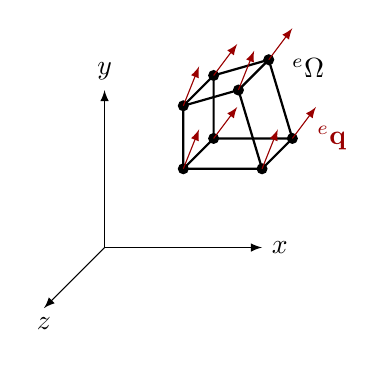
\begin{tikzpicture}
        \draw[-latex] (1,1,1) -- (3,1,1) node[right]{$x$};
        \draw[-latex] (1,1,1) -- (1,3,1) node[above]{$y$};
        \draw[-latex] (1,1,1) -- (1,1,3) node[below]{$z$};
        % Label the region Omega	
        \node at (3.2,2.9) {${}^e\Omega$};
        % Label the boundary Gamma
        \draw[thick] (2,2,1) -- (2,2.8,1) -- (2.7,3,1) -- (3,2,1) -- cycle;
        \draw[thick] (2,2,0) -- (2,2.8,0) -- (2.7,3,0) -- (3,2,0) -- cycle;
        \draw[thick] (2,2,1) -- (2,2,0);
        \draw[thick] (2,2.8,1) -- (2,2.8,0);
        \draw[thick] (2.7,3,1) -- (2.7,3,0);
        \draw[thick] (3,2,1) -- (3,2,0);
        % Fill vertices
        \foreach \point in {(2,2,1), (2,2.8,1), (2.7,3,1), (3,2,1)} {
            \fill \point circle (2pt);
            \draw[-latex, darkred] \point -- ++ (0.2,0.5,0);
          }
        \foreach \point in {(2,2,0), (2,2.8,0), (2.7,3,0), (3,2,0)} {
            \fill \point circle (2pt);
            \draw[-latex, darkred] \point -- ++ (0.3,0.4,0);
          }
        \node[darkred] at (3.5,2) {${^e}\mathbf q$};
      \end{tikzpicture}
      \vfill
    \end{column}
    \begin{column}{.6\textwidth}
      \vspace{-1cm}
      \begin{block}{}
        $${^e}\mathbf u^{h}
          =\left[
            \begin{array}{c;{2pt/2pt}c;{2pt/2pt}c;{2pt/2pt}c}
              {}^eh_{1}\mathbf I & {}^eh_{2}\mathbf I & \dots & {}^eh_{{}^ep}\mathbf I \\
            \end{array} \right]
          \begin{pmatrix}
            {}^e\mathbf q_{1}     \\
            {}^e\mathbf q_{2}     \\
            \vdots                \\
            {}^e\mathbf q_{{}^ep} \\
          \end{pmatrix}
        $$\vspace{0.3cm}
        $${^e}\bolddelta\mathbf u^{h}
          =\left[
            \begin{array}{c;{2pt/2pt}c;{2pt/2pt}c;{2pt/2pt}c}
              {}^eh_{1}\mathbf I & {}^eh_{2}\mathbf I & \dots & {}^eh_{{}^ep}\mathbf I \\
            \end{array} \right]
          \begin{pmatrix}
            {}^e\bolddelta\mathbf q_{1}     \\
            {}^e\bolddelta\mathbf q_{2}     \\
            \vdots                          \\
            {}^e\bolddelta\mathbf q_{{}^ep} \\
          \end{pmatrix}
        $$
      \end{block}
    \end{column}
  \end{columns}
\end{frame}


\begin{frame}{Localisation matrices}
  \begin{center}
    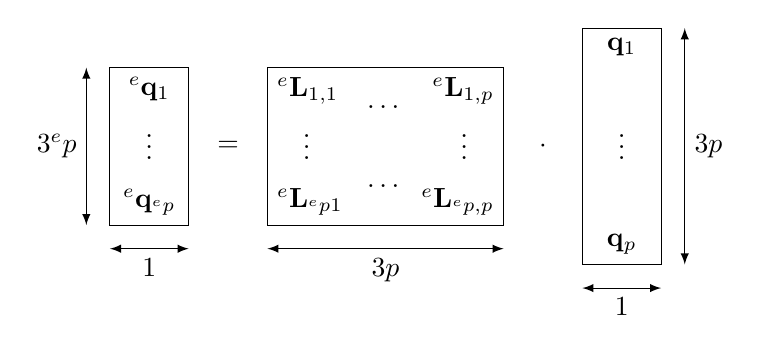
\begin{tikzpicture}
      % First rectangle
      \draw (0,0) rectangle (1,2);
      \node[above] at (0.5,0) {${}^e\mathbf q_{^ep}$};
      \node at (0.5,1.1) {$\vdots$};
      \node[below] at (0.5,2) {${}^e\mathbf q_1$};
      % Dimension labels for first rectangle
      \draw[latex-latex] (-0.3,0) -- (-0.3,2);
      \node[left] at (-0.3,1) {$3^ep$};
      \draw[latex-latex] (0,-0.3) -- (1,-0.3);
      \node[below] at (0.5,-0.3) {$1$};
      % Equal sign
      \node at (1.5,1) {$=$};
      % Second rectangle 
      \draw (2,0) rectangle (5,2);
      \node[above right] at (2,0) {${}^e\mathbf L_{^ep1}$};
      \node[above left] at (5,0) {${}^e\mathbf L_{^ep,p}$};
      \node[below right] at (2,2) {${}^e\mathbf L_{1,1}$};
      \node[below left] at (5,2) {${}^e\mathbf L_{1,p}$};
      \node at (3.5,0.5) {$\dots$};
      \node at (3.5,1.5) {$\dots$};
      \node at (2.5,1.1) {$\vdots$};
      \node at (4.5,1.1) {$\vdots$};

      % Dimension labels for second rectangle
      \draw[latex-latex] (2,-0.3) -- (5,-0.3);
      \node[below] at (3.5,-0.3) {$3p$};

      \node at (5.5,1) {$\cdot$};

      % Third rectangle: 3m x 1
      \draw (6,-0.5) rectangle (7,2.5);
      \node[above] at (6.5,-0.5) {$\mathbf q_{p}$};
      \node at (6.5,1.1) {$\vdots$};
      \node[below] at (6.5,2.5) {$\mathbf q_1$};

      % Dimension labels for third rectangle
      \draw[latex-latex] (7.3,-0.5) -- (7.3,2.5);
      \node[right] at (7.3,1) {$3p$};
      \draw[latex-latex] (6,-0.8) -- (7,-0.8);
      \node[below] at (6.5,-0.8) {$1$};
    \end{tikzpicture}
  \end{center}
  \vspace{-.5cm}
  \begin{block}{}
    \centering $^e\mathbf q={}^e\mathbf L\mathbf q$
  \end{block}
  $^e\mathbf L$ is a Boolean location matrix:
  \begin{itemize}
    \item $^e\mathbf L_{ij}=\mathbf I$ ($3\times 3$ identity matrix) if global node $j$ corresponds to local node $i$,
    \item $^e\mathbf L_{ij}=\mathbf 0$ ($3\times 3$ null matrix) otherwise.
  \end{itemize}
\end{frame}

\begin{frame}{Localization matrices - example}
  \vspace{-1cm}
  \begin{columns}[T]
    \begin{column}{.4\textwidth}
      \begin{center}
        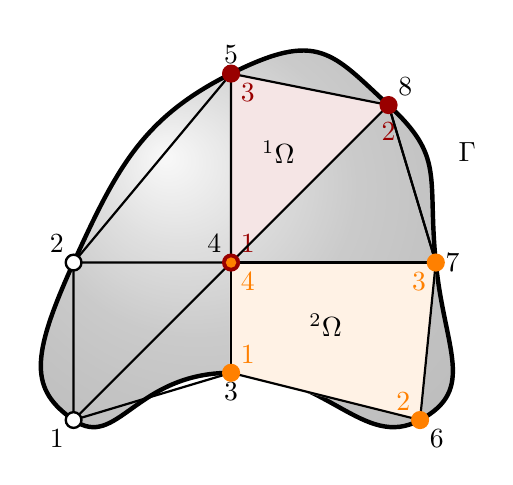
\begin{tikzpicture}[scale=2]
          % \draw[step=1.0,black,thin] (0,0) grid (4,4);
          % Draw the potato-like shape
          \shade [ball color= gray!90!black, opacity=.3] plot [thick,smooth cycle, tension=1] coordinates  {(1,2) (2,3.2) (3,3) (3.3,2) (3.2,1) (2,1.3) (1,1)};
          \draw[ultra thick] plot [thick,smooth cycle, tension=1] coordinates {(1,2) (2,3.2) (3,3) (3.3,2) (3.2,1) (2,1.3) (1,1)};
          \draw[fill=darkred!30,thick,darkred!10] (2,2) -- (3,3) -- (2,3.2) -- cycle;
          \draw[fill=orange!30,thick,orange!10] (2,2) -- (3.3,2) -- (3.2,1) -- (2,1.3) -- cycle;
          % label the nodes
          \node[below left] at (1,1) {$1$};
          \node[above left] at (1,2) {$2$};
          \node[below] at (2,1.3) {$3$};
          \node[orange,above right] at (2,1.3) {$1$};
          \node[above left] at (2,2) {$4$};
          \node[darkred,above right] at (2,2) {$1$};
          \node[orange,below right] at (2,2) {$4$};
          \node[above] at (2,3.2) {$5$};
          \node[darkred,below right] at (2,3.2) {$3$};
          \node[below right] at (3.2,1) {$6$};
          \node[orange,above left] at (3.2,1) {$2$};
          \node[right] at (3.3,2) {$7$};
          \node[orange,below left] at (3.3,2) {$3$};
          \node[above right] at (3,3) {$8$};
          \node[darkred,below={3pt}] at (3,3) {$2$};
          % Label the region Omega
          \node at (2.3,2.7) {${}^1\Omega$};
          \node at (2.6,1.6) {${}^2\Omega$};
          % Label the boundary Gamma
          \node at (3.5,2.7) {$\Gamma$};
          \draw[thick] (1,2) -- (2,3.2) -- (3,3) -- (3.3,2) -- (3.2,1) -- (2,1.3) -- (1,1) -- cycle;
          \draw[thick] (1,2) -- (2,2) -- (3,3) -- (3.3,2);
          \draw[thick] (2,1.3) -- (2,2) -- (3.3,2);
          \draw[thick] (1,1) -- (2,2) -- (2,2.3) -- (2,3.2);
          \node[darkred,draw,shape=circle,fill=darkred,minimum size=2mm,line width=0.3mm,inner sep=0] at (2,2) {};
          \node[orange,draw,shape=circle,fill=orange,minimum size=1mm,line width=0.3mm,inner sep=0] at (2,2) {};
          \node[draw,shape=circle,fill=white,minimum size=2mm,line width=0.3mm,inner sep=0] at (1,1) {};
          \node[draw,shape=circle,fill=white,minimum size=2mm,line width=0.3mm,inner sep=0] at (1,2) {};
          \node[orange,draw,shape=circle,fill=orange,minimum size=2mm,line width=0.3mm,inner sep=0] at (2,1.3) {};
          \node[darkred,draw,shape=circle,fill=darkred,minimum size=2mm,line width=0.3mm,inner sep=0] at (2,3.2) {};
          \node[darkred,draw,shape=circle,fill=darkred,minimum size=2mm,line width=0.3mm,inner sep=0] at (3,3) {};
          \node[orange,draw,shape=circle,fill=orange,minimum size=2mm,line width=0.3mm,inner sep=0] at (3.2,1) {};
          \node[orange,draw,shape=circle,fill=orange,minimum size=2mm,line width=0.3mm,inner sep=0] at (3.3,2) {};
        \end{tikzpicture}
      \end{center}
    \end{column}
    \begin{column}{.6\textwidth}
      \vspace{0.5cm}
      \begin{itemize}
        \item Number of nodes in the mesh: $p=8$.
        \item Number of elements in the mesh: $m=6$.
        \item Number of nodes in the element ${}^1\Omega$: ${}^1p=3$.
              $${}^1\mathbf L=
                \begin{bmatrix}
                  \mathbf 0 & \mathbf 0 & \mathbf 0 & \mathbf I & \mathbf 0 & \mathbf 0 & \mathbf 0 & \mathbf 0 & \\
                  \mathbf 0 & \mathbf 0 & \mathbf 0 & \mathbf 0 & \mathbf 0 & \mathbf 0 & \mathbf 0 & \mathbf I & \\
                  \mathbf 0 & \mathbf 0 & \mathbf 0 & \mathbf 0 & \mathbf I & \mathbf 0 & \mathbf 0 & \mathbf 0 & \\
                \end{bmatrix}$$
        \item Number of nodes in the element ${}^2\Omega$: ${}^2p=4$.
              $${}^2\mathbf L=
                \begin{bmatrix}
                  \mathbf 0 & \mathbf 0 & \mathbf I & \mathbf 0 & \mathbf 0 & \mathbf 0 & \mathbf 0 & \mathbf 0 & \\
                  \mathbf 0 & \mathbf 0 & \mathbf 0 & \mathbf 0 & \mathbf 0 & \mathbf I & \mathbf 0 & \mathbf 0 & \\
                  \mathbf 0 & \mathbf 0 & \mathbf 0 & \mathbf 0 & \mathbf 0 & \mathbf 0 & \mathbf I & \mathbf 0 & \\
                  \mathbf 0 & \mathbf 0 & \mathbf 0 & \mathbf I & \mathbf 0 & \mathbf 0 & \mathbf 0 & \mathbf 0 & \\
                \end{bmatrix}$$
      \end{itemize}
    \end{column}
  \end{columns}
\end{frame}

\begin{frame}{Localisation matrices - memory usage}
  \begin{columns}
    \column{0.4\textwidth}
    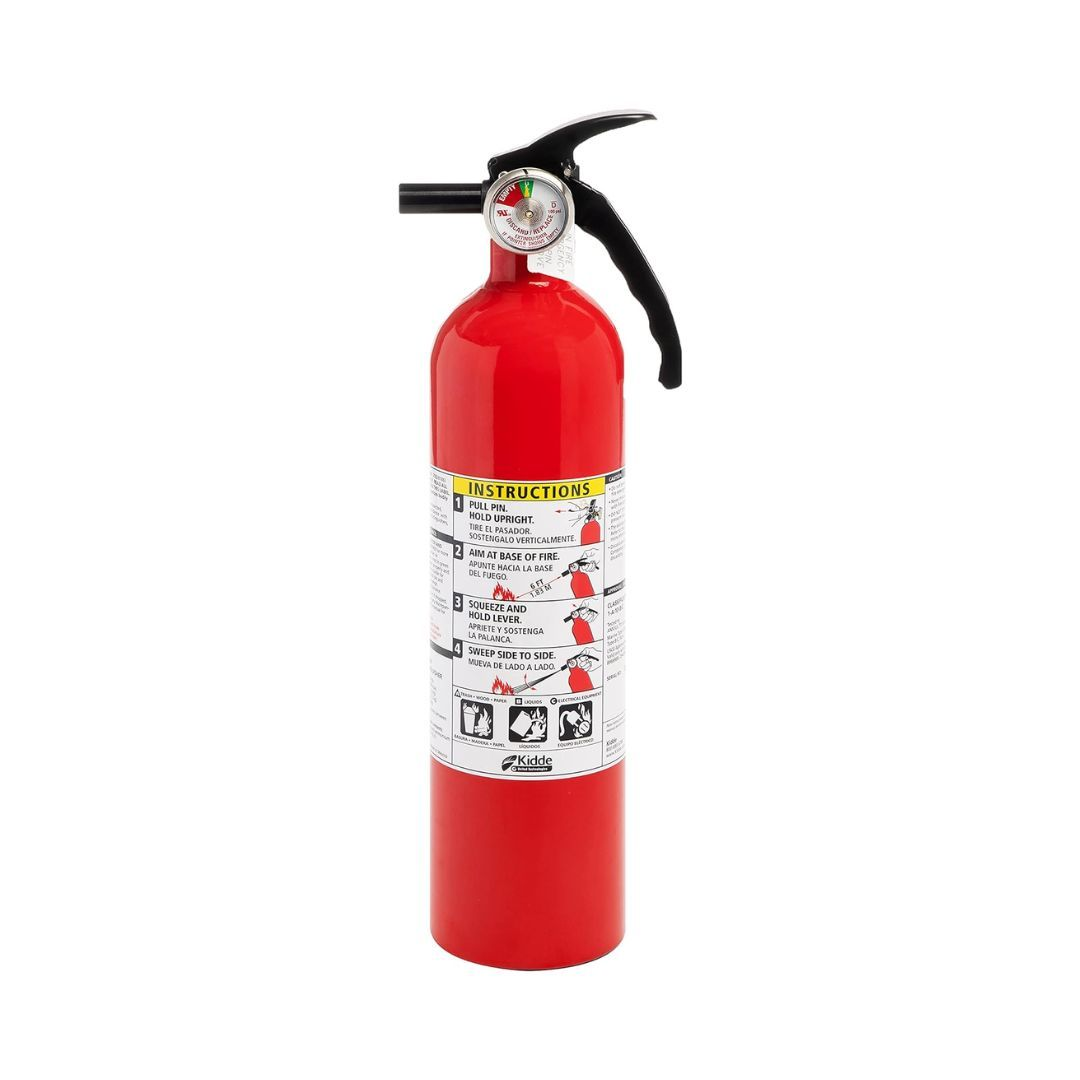
\includegraphics[width=\linewidth]{../images/fireextinguisher.jpg}
    \column{0.6\textwidth}
    \textbf{Practical example:} \\[5pt] Consider a mesh made of
    \begin{itemize}
      \item $p=10'000$ nodes,
      \item trilinear hexahedral finite elements with $^ep=8$ nodes each.
    \end{itemize}
    \emph{Every} localization matrix \( ^e\mathbf{L} \) contains
    \begin{itemize}
      \item $720'000$ entries,
      \item of which \( 3^e p = 24 \) are 1s,
      \item the remaining $719'976$ are 0s.
    \end{itemize}
  \end{columns}
\end{frame}

\begin{frame}{Connectivity table: local to global node numbering}
  \begin{itemize}
    \item Elements and their connectivity are defined using a table.
    \item Example of connectivity table:
  \end{itemize}
  \vspace{0.2cm}
  \[
    \begin{array}{c|cccc}
      ^e\Omega & ^1\Omega & ^2\Omega & ^3\Omega & ^4\Omega \\
      \hline
      1        & 1        & 2        & 4        & 5        \\
      2        & 2        & 3        & 5        & 6        \\
      3        & 5        & 6        & 8        & 9        \\
      4        & 4        & 5        & 7        & 8        \\
    \end{array}
  \]
  \vspace{0.2cm}
  \begin{itemize}
    \item The connectivity table provides the global numbering for each node in each element, corresponding to a column in the table above.
    \item The localization matrices \( ^e\mathbf{L} \) can be constructed from the connectivity table.
  \end{itemize}
\end{frame}

\begin{frame}{Additivity of integrals}
  \begin{itemize}
    \item  Approximated weak form:
          $${\color{brown}\int_{\Omega} (\boldsymbol{\nabla} \bolddelta\mathbf u^{h} )^{T} \mathbf C\boldsymbol{\nabla} \mathbf u^{h}\, d\Omega}+{\color{darkred}\int_{\Omega} \rho(\bolddelta\mathbf u^{h})^{T}\mathbf{\ddot{u}}^{h}\, d\Omega}= {\color{orange}\int_{\Gamma_\sigma} (\bolddelta\mathbf u^{h})^{T}\mathbf{\hat f} \, d\Gamma+\int_{\Omega}  (\bolddelta\mathbf u^{h})^{T}\mathbf f\, d\Omega}$$
    \item  We localize the integrals using their additivity property:
          \begin{align*}
              & \sum_{e=1}^m\left({\color{brown}\int_{{}^e\Omega} (\boldsymbol{\nabla} {}^e\bolddelta\mathbf u^{h} )^{T} \mathbf C\boldsymbol{\nabla} {}^e\mathbf u^{h}\, d\Omega}+{\color{darkred}\int_{{}^e\Omega} \rho({}^e\bolddelta\mathbf u^{h})^{T}{}^e\mathbf{\ddot{u}}^{h}\, d\Omega}\right) \\
            = & \sum_{e=1}^m\left({\color{orange}\int_{{}^e\Gamma_\sigma} ({}^e\bolddelta\mathbf u^{h})^{T}\mathbf{\hat f} \, d\Gamma+\int_{{}^e\Omega}  ({}^e\bolddelta\mathbf u^{h})^{T}\mathbf f\, d\Omega}\right)
          \end{align*}
          and consider the local quantities $^e\mathbf u^h={}^e\mathbf H{}^e\mathbf L \mathbf q$ and ${}^e \bolddelta \mathbf{u}^h = {}^e\mathbf{H}{}^e\mathbf L \bolddelta\mathbf{q}$.
  \end{itemize}
\end{frame}

\begin{frame}{Additivity of integrals - inertial forces}
  Recall $^e\mathbf u^h={}^e\mathbf H{}^e\mathbf L \mathbf q$ and ${}^e \bolddelta \mathbf{u}^h = {}^e\mathbf{H}{}^e\mathbf L \bolddelta\mathbf{q}$.
  \vspace{0.5cm}
  \begin{enumerate}
    \item  Consider only the term related to the virtual work of inertial forces (acceleration):
          \[
            \sum_{e=1}^m {\color{darkred}\int_{{}^e\Omega}\rho({}^e\bolddelta\mathbf u^{h})^{T}{}^e\mathbf{\ddot{u}}^{h}\, d\Omega}  =\bolddelta\mathbf{q}^T \Big[\sum_{e=1}^m {}^e\mathbf L^T\Big(\underbrace{\int_{{}^e\Omega} \rho{}^e\mathbf H^{T}{}^e\mathbf H\, d\Omega}_\text{${}^e\mathbf M$}\Big) {}^e\mathbf L\Big] \mathbf{\ddot{q}}
          \]
  \end{enumerate}
\end{frame}

\begin{frame}{Additivity of integrals - internal and external forces}
  Recall $^e\mathbf u^h={}^e\mathbf H{}^e\mathbf L \mathbf q$ and ${}^e \bolddelta \mathbf{u}^h = {}^e\mathbf{H}{}^e\mathbf L \bolddelta\mathbf{q}$.
  \vspace{0.5cm}
  \begin{enumerate}
    \setcounter{enumi}{1}
    \item  Analogously for the term related to the virtual work of internal forces:
          \[
            \sum_{e=1}^m {\color{brown}\int_{{}^e\Omega} (\boldsymbol{\nabla} {}^e\bolddelta\mathbf u^{h} )^{T} \mathbf C\boldsymbol{\nabla} {}^e\mathbf u^{h}\, d\Omega }=\bolddelta\mathbf{q}^T \Big[\sum_{e=1}^m {}^e\mathbf L^T\Big(\underbrace{\int_{{}^e\Omega}\boldsymbol{\nabla}{}^e\mathbf H^{T}\mathbf C\boldsymbol{\nabla}{}^e\mathbf H\, d\Omega}_\text{${}^e\mathbf K$}\Big) {}^e\mathbf L\Big] \mathbf{q}
          \]
    \item  Term realted to the virtual work of external forces:
          \begin{align*}
             & \sum_{e=1}^m {\color{orange}\int_{{}^e\Gamma_\sigma} ({}^e\bolddelta\mathbf u^{h})^{T}\mathbf{\hat f} \, d\Gamma+\int_{{}^e\Omega}  ({}^e\bolddelta\mathbf u^{h})^{T}\mathbf f\, d\Omega} \\                                                                  =\bolddelta\mathbf{q}^T &\sum_{e=1}^m {}^e\mathbf L^T\Big(\underbrace{\int_{{}^e\Gamma_\sigma} {}^e\mathbf H^{T}\mathbf{\hat f} \, d\Gamma+\int_{{}^e\Omega} {}^e\mathbf H^{T}\mathbf f\, d\Omega }_\text{${}^e\mathbf r(t)$}\Big)
          \end{align*}
  \end{enumerate}
\end{frame}


{\setbeamercolor{background canvas}{bg=darkred}
\setbeamercolor{block body}{bg=darkred,fg=white}
\setbeamercolor{itemize item}{fg=white}
\begin{frame}{Elementary matrices and vectors}
  \begin{block}{}
    \begin{itemize}
      \item \textbf{Elementary stiffness matrix} ($3{}^e p\times 3{}^e p$):
            $${}^e\mathbf K=\int_{{}^e\Omega} {}^e\mathbf B^T\mathbf C{}^e\mathbf B \, d\Omega$$
            ${}^e\mathbf B=\boldsymbol{\nabla} {}^e\mathbf H=\left[
                \begin{array}{c;{2pt/2pt}c;{2pt/2pt}c}
                  \boldsymbol{\nabla} {}^eh_1 & \dots & \boldsymbol{\nabla} {}^eh_{{}^ep}
                \end{array} \right]$
            elementary deformation matrix ($6\times 3{}^e p$) .
      \item \textbf{Elementary mass matrix} ($3{}^e p\times 3{}^e p$):
            $${}^e\mathbf M=\int_{{}^e\Omega} \rho\, {}^e\mathbf H^T{}^e\mathbf H \, d\Omega.$$
      \item \textbf{Elementary applied forces vector} ($3{}^e p\times 1$):
            $${}^e\mathbf r(t)=\int_{{}^e\Gamma_\sigma} {}^e\mathbf H^{T}\mathbf{\hat f} \, d\Gamma+\int_{{}^e\Omega} {}^e\mathbf H^{T}\mathbf f\, d\Omega.$$
    \end{itemize}
  \end{block}
\end{frame}

\begin{frame}{Assembly operator}
  \begin{block}{}
    We define the assembly operator as follows:
    \begin{align*}
      \mathbf K & =\A_{e=1}^m {}^e\mathbf K = \sum_{e=1}^{m} {}^e\mathbf L^T {}^e\mathbf K{}^e\mathbf L \\[10pt]
      \mathbf M & =\A_{e=1}^m {}^e\mathbf M = \sum_{e=1}^{m} {}^e\mathbf L^T {}^e\mathbf M{}^e\mathbf L \\[10pt]
      \mathbf r & =\A_{e=1}^m {}^e\mathbf r = \sum_{e=1}^{m} {}^e\mathbf L^T {}^e\mathbf r{}            \\
    \end{align*}
  \end{block}
\end{frame}
}

\section{Automating integration and archetypal shape functions}

 {\usebackgroundtemplate{
\includegraphics[height=\paperheight]{../images/inception.jpg}}%
  \begin{frame}{Elements}
    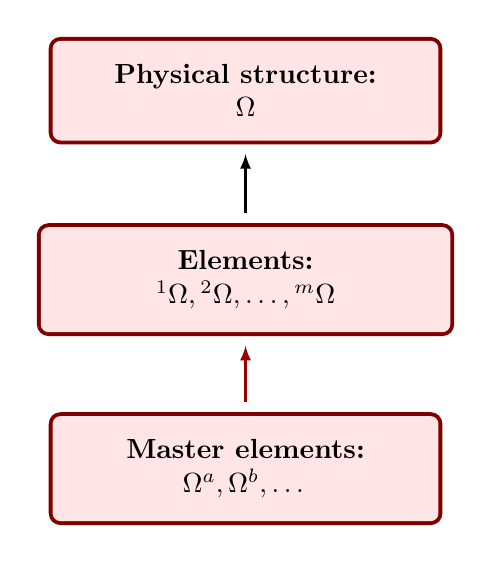
\begin{tikzpicture}[scale=0.8]
      \node (pe) at (-2,6) {
        \begin{tcolorbox}[colframe=red!50!black, colback=red!10, coltitle=black, rounded corners, width=5cm]
          \centering \textbf{Physical structure:} \\ $\Omega$
        \end{tcolorbox}
      };
      \node (ee) at (-2,3) {
        \begin{tcolorbox}[colframe=red!50!black, colback=red!10, coltitle=black, rounded corners,width=5.3cm]
          \centering \textbf{Elements:} \\ ${}^1\Omega,{}^2\Omega,\dots, {}^m\Omega$
        \end{tcolorbox}
      };
      \node (me) at (-2,0) {
        \begin{tcolorbox}[colframe=red!50!black, colback=red!10, coltitle=black, rounded corners,width=5cm]
          \centering \textbf{Master elements:} \\ $\Omega^a,\Omega^b,\dots$
        \end{tcolorbox}
      };
      % Drawing arrows
      \draw[latex-, thick] (pe.south) -- (ee.north);
      \draw[latex-, thick, darkred] (ee.south) -- (me.north);
    \end{tikzpicture}
  \end{frame}
 }

 {\setbeamercolor{background canvas}{bg=darkred}
  \setbeamercolor{block body}{bg=darkred,fg=white}
  \setbeamercolor{itemize item}{fg=white}
  \begin{frame}{Coordinate transform}
    \begin{block}{}
      To automate the integration and simplify the definition of shape functions, we transform each \emph{distorted} finite element ${}^e\Omega$ into a \textbf{reference (archetypal or master) element} $\Omega^a$ where we can apply standard numerical integration schemes.
      \begin{itemize}
        \item The coordinate transformation:
              \begin{align*}
                {}^eT : \Omega^a & \to {}^e\Omega             \\
                \boldxi          & \mapsto \mathbf x(\boldxi)
              \end{align*}
              maps any point $\boldxi = \{\xi_1, \xi_2, \xi_3\}^T$ in $\Omega^a$ to its corresponding point of coordinate $\mathbf x = \mathbf x(\boldxi)= \{x_1(\boldxi), x_2(\boldxi), x_3(\boldxi)\}^T$ in ${}^e\Omega$.
        \item  ${}^eT$ is a bijective application.
      \end{itemize}
    \end{block}
  \end{frame}
 }

\begin{frame}{An illustration of a coordinate transform ${}^eT$ in 3D}
  \begin{center}
    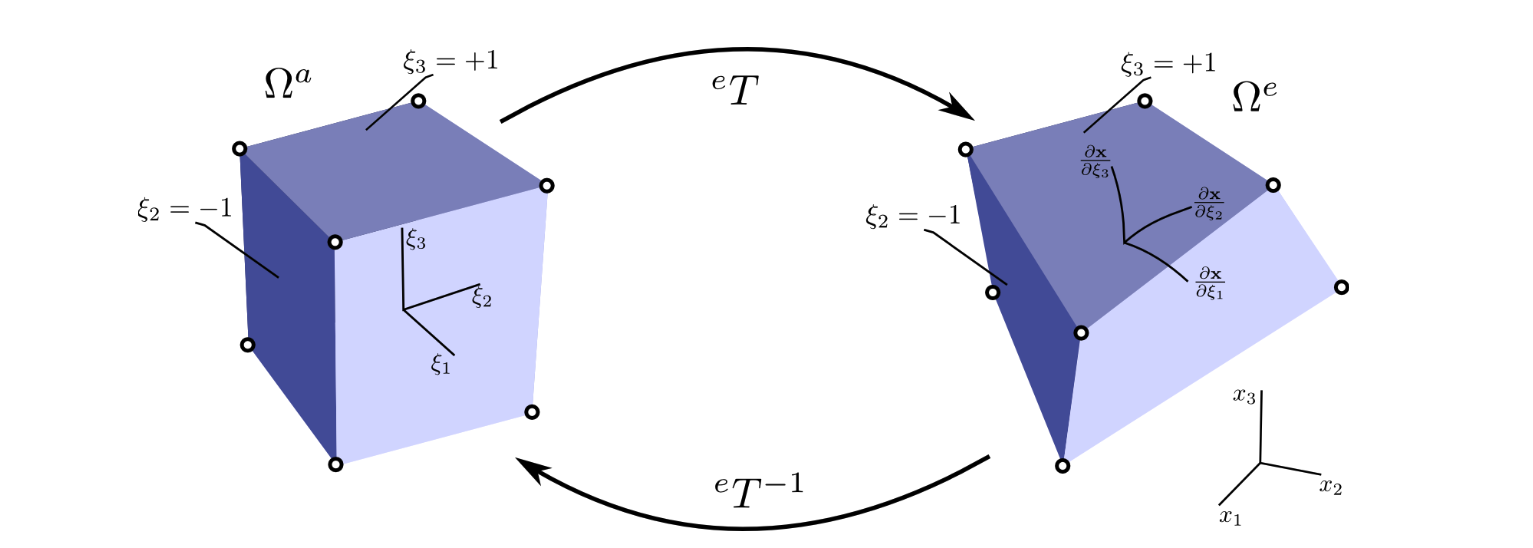
\includegraphics[width=\textwidth]{../images/coordTrans.png}
  \end{center}
  {\footnotesize (Credit: Joel Cugnoni - Finite Element Method applied to linear statics of deformable solids)}
\end{frame}

\begin{frame}{An illustration of coordinate transforms in 2D}
  \begin{center}
    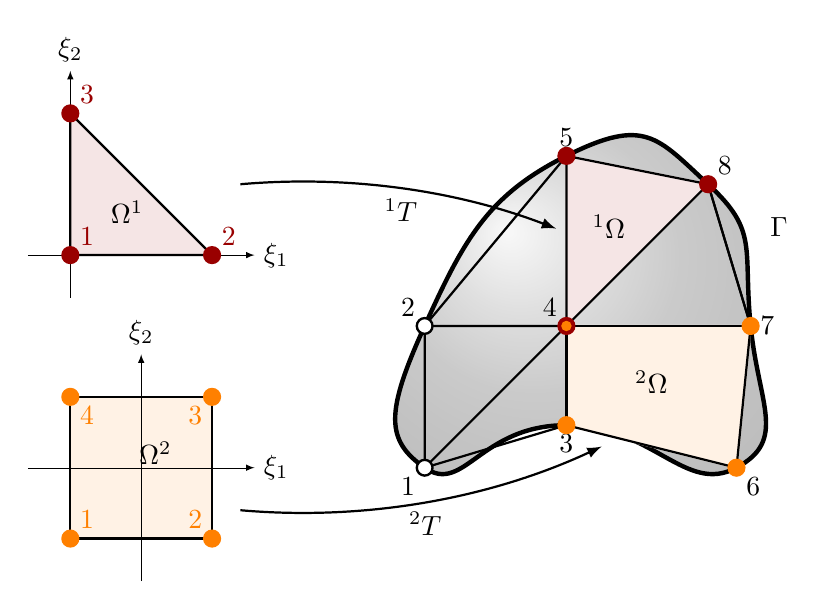
\begin{tikzpicture}[scale=1.8]
      % \draw[step=1.0,black,thin] (-2,0) grid (4,4);
      % Draw the potato-like shape
      \shade [ball color= gray!90!black, opacity=.3] plot [thick,smooth cycle, tension=1] coordinates  {(1,2) (2,3.2) (3,3) (3.3,2) (3.2,1) (2,1.3) (1,1)};
      \draw[ultra thick] plot [thick,smooth cycle, tension=1] coordinates {(1,2) (2,3.2) (3,3) (3.3,2) (3.2,1) (2,1.3) (1,1)};
      \draw[fill=darkred!30,thick,darkred!10] (2,2) -- (3,3) -- (2,3.2) -- cycle;
      \draw[fill=orange!30,thick,orange!10] (2,2) -- (3.3,2) -- (3.2,1) -- (2,1.3) -- cycle;
      % label the nodes
      \node[below left] at (1,1) {$1$};
      \node[above left] at (1,2) {$2$};
      \node[below] at (2,1.3) {$3$};
      \node[above left] at (2,2) {$4$};
      \node[above] at (2,3.2) {$5$};
      \node[below right] at (3.2,1) {$6$};
      \node[right] at (3.3,2) {$7$};
      \node[above right] at (3,3) {$8$};
      % Label the region Omega
      \node at (2.3,2.7) {${}^1\Omega$};
      \node at (2.6,1.6) {${}^2\Omega$};
      % Label the boundary Gamma
      \node at (3.5,2.7) {$\Gamma$};
      \draw[thick] (1,2) -- (2,3.2) -- (3,3) -- (3.3,2) -- (3.2,1) -- (2,1.3) -- (1,1) -- cycle;
      \draw[thick] (1,2) -- (2,2) -- (3,3) -- (3.3,2);
      \draw[thick] (2,1.3) -- (2,2) -- (3.3,2);
      \draw[thick] (1,1) -- (2,2) -- (2,2.3) -- (2,3.2);
      \node[darkred,draw,shape=circle,fill=darkred,minimum size=2mm,line width=0.3mm,inner sep=0] at (2,2) {};
      \node[orange,draw,shape=circle,fill=orange,minimum size=1mm,line width=0.3mm,inner sep=0] at (2,2) {};
      \node[draw,shape=circle,fill=white,minimum size=2mm,line width=0.3mm,inner sep=0] at (1,1) {};
      \node[draw,shape=circle,fill=white,minimum size=2mm,line width=0.3mm,inner sep=0] at (1,2) {};
      \node[orange,draw,shape=circle,fill=orange,minimum size=2mm,line width=0.3mm,inner sep=0] at (2,1.3) {};
      \node[darkred,draw,shape=circle,fill=darkred,minimum size=2mm,line width=0.3mm,inner sep=0] at (2,3.2) {};
      \node[darkred,draw,shape=circle,fill=darkred,minimum size=2mm,line width=0.3mm,inner sep=0] at (3,3) {};
      \node[orange,draw,shape=circle,fill=orange,minimum size=2mm,line width=0.3mm,inner sep=0] at (3.2,1) {};
      \node[orange,draw,shape=circle,fill=orange,minimum size=2mm,line width=0.3mm,inner sep=0] at (3.3,2) {};
      % Draw master square
      \draw[fill=orange!30,thick,orange!10] (-1.5,0.5) -- (-0.5,0.5) -- (-0.5,1.5) -- (-1.5,1.5) -- cycle;
      \draw[thick] (-1.5,0.5) -- (-0.5,0.5) -- (-0.5,1.5) -- (-1.5,1.5) -- cycle;
      \draw[ultra thin,-latex] (-1.8,1) -- (-0.2,1) node[right]{$\xi_1$};
      \draw[ultra thin,-latex] (-1,0.2) -- (-1,1.8) node[above]{$\xi_2$};
      \node at (-0.9,1.1) {$\Omega^2$};
      \draw[thick,-latex] (-0.3,0.7) arc [start angle=-95, end angle=-65, radius=5] node[midway, below]{${}^2T$};
      \node[orange,draw,shape=circle,fill=orange,minimum size=2mm,line width=0.3mm,inner sep=0] at (-1.5,0.5) {};
      \node[orange,draw,shape=circle,fill=orange,minimum size=2mm,line width=0.3mm,inner sep=0] at (-0.5,0.5) {};
      \node[orange,draw,shape=circle,fill=orange,minimum size=2mm,line width=0.3mm,inner sep=0] at (-0.5,1.5) {};
      \node[orange,draw,shape=circle,fill=orange,minimum size=2mm,line width=0.3mm,inner sep=0] at (-1.5,1.5) {};
      \node[orange,above right] at (-1.5,0.5) {$1$};
      \node[orange,below right] at (-1.5,1.5) {$4$};
      \node[orange,above left] at (-0.5,0.5) {$2$};
      \node[orange,below left] at (-0.5,1.5) {$3$};
      % Draw master triangle
      \draw[fill=darkred!30,thick,darkred!10] (-1.5,2.5) -- (-0.5,2.5) -- (-1.5,3.5) -- cycle;
      \draw[thick] (-1.5,2.5) -- (-0.5,2.5) -- (-1.5,3.5) -- cycle;
      \draw[ultra thin,-latex] (-1.8,2.5) -- (-0.2,2.5) node[right]{$\xi_1$};
      \draw[ultra thin,-latex] (-1.5,2.2) -- (-1.5,3.8) node[above]{$\xi_2$};
      \node[darkred,draw,shape=circle,fill=darkred,minimum size=2mm,line width=0.3mm,inner sep=0] at (-1.5,2.5) {};
      \node[darkred,draw,shape=circle,fill=darkred,minimum size=2mm,line width=0.3mm,inner sep=0] at (-0.5,2.5) {};
      \node[darkred,draw,shape=circle,fill=darkred,minimum size=2mm,line width=0.3mm,inner sep=0] at (-1.5,3.5) {};
      \node[darkred,above right] at (-1.5,2.5) {$1$};
      \node[darkred,above right] at (-0.5,2.5) {$2$};
      \node[darkred,above right] at (-1.5,3.5) {$3$};
      \node at (-1.1,2.8) {$\Omega^1$};
      \draw[thick,-latex] (-0.3,3) arc [start angle=95, end angle=69, radius=5] node[midway, below]{${}^1T$};
    \end{tikzpicture}
  \end{center}
\end{frame}

\begin{frame}{Biunivocity of coordinate transformation ${}^eT$}
  \begin{block}{}
    $$
      ^{e} \mathbf{J} =
      \begin{bmatrix}
        \frac{\partial x_1}{\partial \xi_1} & \frac{\partial x_1}{\partial \xi_2} & \frac{\partial x_1}{\partial \xi_3} \\[5pt]
        \frac{\partial x_2}{\partial \xi_1} & \frac{\partial x_2}{\partial \xi_2} & \frac{\partial x_2}{\partial \xi_3} \\[5pt]
        \frac{\partial x_3}{\partial \xi_1} & \frac{\partial x_3}{\partial \xi_2} & \frac{\partial x_3}{\partial \xi_3}
      \end{bmatrix}\hspace{1.5cm}
      {}^{e} \mathbf{J}^{-1} =
      \begin{bmatrix}
        \frac{\partial \xi_1}{\partial x_1} & \frac{\partial \xi_1}{\partial x_2} & \frac{\partial \xi_1}{\partial x_3} \\[5pt]
        \frac{\partial \xi_2}{\partial x_1} & \frac{\partial \xi_2}{\partial x_2} & \frac{\partial \xi_3}{\partial x_3} \\[5pt]
        \frac{\partial \xi_3}{\partial x_1} & \frac{\partial \xi_3}{\partial x_2} & \frac{\partial \xi_3}{\partial x_3}
      \end{bmatrix}
    $$
    \begin{itemize}
      \item \({}^{e} \mathbf{J}\) is the Jacobian matrix associated with  \({}^{e}T\):  ${}^e\mathbf{J}_{ij} = \frac{\partial x_i}{\partial \xi_j}$ $(i,j=1,2,3)$,
      \item   \({}^{e} \mathbf{J}^{-1}\) is the inverse Jacobian matrix,
      \item  \( {}^e j =\det({}^{e} \mathbf{J})\) is the determinant of the Jacobian matrix \( {}^e \mathbf{J} \).
    \end{itemize}
    \vspace{0.3cm}
    \textbf{Sufficient condition for invertibility}: if ${}^{e} j>0$ everywhere in ${}^e\Omega$, then  \({}^{e}T\) is invertible in ${}^e\Omega$ and \({}^{e} \mathbf{J}^{-1}\) exists.
  \end{block}

\end{frame}

\begin{frame}{Master elements and master shape functions}
  \begin{itemize}
    \item The coordinate transformation  \({}^eT^{-1} \) maps shape functions on  \( {}^e\Omega \) to the master element space \( \Omega^a \):
          \[
            {}^a\mathbf H(\boldxi)={}^e\mathbf H(\mathbf x(\boldxi))
          \]
    \item Inside each element \( {}^e\Omega \):
          \[
            {}^e\mathbf u^h[\mathbf x(\boldxi)] = {}^a\mathbf H(\boldxi) {}^e \mathbf q
          \]
    \item This allows shape function \( {}^a\mathbf H(\boldxi) \) to be defined only \emph{once} on each master element \({}^a \Omega \).
    \item[\HandRight] \textbf{{\color{darkred}Result}: master shape functions!}
  \end{itemize}
\end{frame}

\begin{frame}{An illustration of a master shape function}
  \begin{center}
    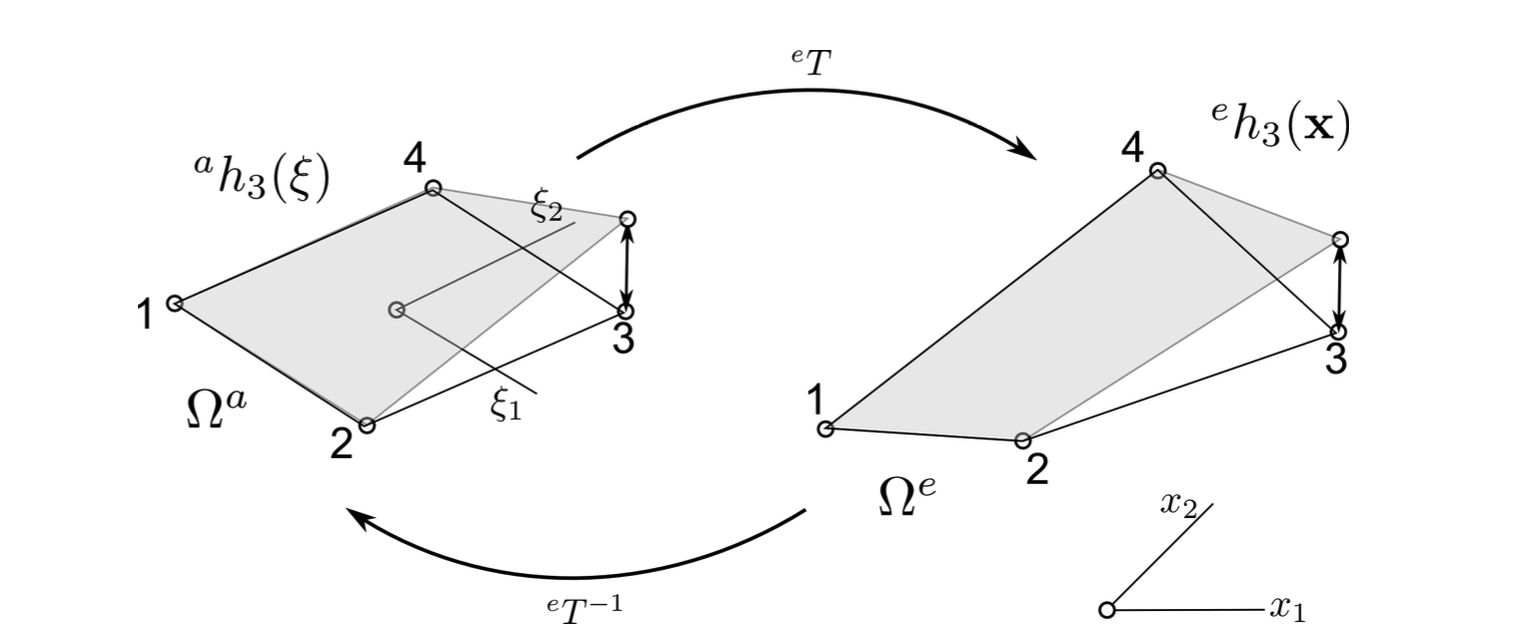
\includegraphics[width=\textwidth]{../images/masterShapeFunction.png}
  \end{center}
  {\footnotesize (Credit: Joel Cugnoni - Finite Element Method applied to linear statics of deformable solids)}
\end{frame}

\begin{frame}{Choosing a simple coordinate transformation}
  \begin{itemize}
    \item[\HandRight] Coordinate transformations are defined using the shape functions:
          \[
            {\color{darkred}{}^eT : \mathbf x(\boldxi) = {}^a\mathbf H(\boldxi) ^e{} \mathbf x=\sum_{i=1}^{{}^ep}{}^a h_i(\boldxi){}^e\mathbf x_i       }
          \]
    \item Inside each element \({}^e\Omega \), the local coordinates are interpolated as a linear combination of master shape functions ${}^a h_i$ and nodal coordinates \( {}^e\mathbf  x_i \).
    \item Kronecker property ensures node correspondence: $${}^eh_i(\mathbf x_j) = \delta_{ij}\quad\Rightarrow \quad{}^a h_i(\boldxi_j) = \delta_{ij}.$$
    \item This guarantees that each  node of the master element \( \Omega^a \) maps to a corresponding node in the deformed element \( {}^e\Omega \).
  \end{itemize}
\end{frame}

{\setbeamercolor{background canvas}{bg=darkred!5}
\setbeamercolor{block body}{bg=darkred!5,fg=black}

\begin{frame}{Integration by substitution formulas}
  \begin{itemize}
    \item Given \( {}^eT: \Omega^a \to {}^e\Omega \), an integral over \( {}^e\Omega \) of a function \( F: {}^e\Omega \to \mathbb{R} \) can be rewritten as an integral over \( \Omega^a \):
          \[
            \int_{{}^e\Omega} F(\mathbf{x}) \, d\mathbf x = \int_{\Omega^a} F(\mathbf{x}(\boldsymbol{\xi})) \, {}^e j \, d\boldxi
          \]
    \item When the integrand involves the operator \( \boldsymbol{\nabla} \), then:
          \[
            \int_{{}^e\Omega} \boldsymbol{\nabla}_{\mathbf{x}} F(\mathbf{x}) \, d\mathbf x = \int_{\Omega^a} {}^e\mathbf{J}^{-1}\boldsymbol{\nabla}_{\boldsymbol{\xi}} F(\mathbf{x}(\boldsymbol{\xi}))  \, {}^e j \, d\boldxi
          \]
          since
          \[
            \frac{\partial }{\partial x_i} = \sum_{j=1}^3 \frac{\partial \xi_j}{\partial x_i} \frac{\partial }{\partial \xi_j} =  \sum_{j=1}^3 {}^e\mathbf{J}_{ij}^{-1}\frac{\partial}{\partial \xi_j}.
          \]
  \end{itemize}
\end{frame}
}

\begin{frame}{Master elements and derivatives}
  \begin{itemize}
    \item The spatial derivative operator $\boldsymbol{\nabla}_{\mathbf x}$ is defined in the global coordinate system $(x_1, x_2, x_3)$. Applying the coordinate transform ${}^eT^{-1}$, we can then extend it to be applied on the master element $\Omega^a$:
          \[
            \frac{\partial }{\partial x_i} = \sum_{j=1}^3 \frac{\partial \xi_j}{\partial x_i} \frac{\partial }{\partial \xi_j} =  \sum_{j=1}^3 {}^e\mathbf{J}_{ij}^{-1}\frac{\partial}{\partial \xi_j}.
          \]
    \item The elementary strain-displacement matrix ${}^e\mathbf B$ can be directly derived from the master shape functions ${}^a\mathbf H$:
          \[
            {}^e\mathbf B =\left[\begin{array}{c;{2pt/2pt}c;{2pt/2pt}c}
                \boldsymbol{\nabla}_{\mathbf x} {}^eh_1 & \dots & \boldsymbol{\nabla}_{\mathbf x} {}^eh_{{}^ep}
              \end{array} \right]= \left[\begin{array}{c;{2pt/2pt}c;{2pt/2pt}c}
                {}^e\mathbf J^{-1}\boldsymbol{\nabla}_{\boldxi} {}^ah_1 & \dots & {}^e\mathbf J^{-1}\boldsymbol{\nabla}_{\boldxi} {}^ah_{{}^ep}
              \end{array} \right] .
          \]
  \end{itemize}
\end{frame}

\begin{frame}{Automating the integration}
  Using the coordinate transform ${}^eT$ and master shape functions, the integrals in the definitions of ${}^e\mathbf K$, ${}^e\mathbf M$ and ${}^e\mathbf r$, can be carried out directly on a standard domain $\Omega^a$:
  \begin{align*}
    {}^e\mathbf K    & = \int_{\Omega^a}\left( {}^e{\color{darkred}\mathbf J^{-1}} \boldsymbol{\nabla}_{\boldxi}{}^a\mathbf H \right)^T\mathbf C\left( {}^e{\color{darkred}\mathbf J^{-1}}\boldsymbol{\nabla}_{\boldxi}{}^a\mathbf H \right) \, {\color{darkred}{}^ej} \, d\boldxi \\[12pt]
    {}^e\mathbf M    & =\int_{\Omega^a} \rho\, {}^a\mathbf H^T{}^a\mathbf H \, {\color{darkred}{}^ej} \, d\boldxi                                                                                                                                                                  \\[12pt]
    {}^e\mathbf r(t) & =\int_{\Gamma_\sigma^a} {}^a\mathbf H^{T}\mathbf{\hat f} \,{\color{darkred}{}^ej\big|_{\Gamma_\sigma^a}}\, d\Gamma+\int_{\Omega^a} {}^a\mathbf H^{T}\mathbf f\,{\color{darkred}{}^ej}\, d\boldxi
  \end{align*}
\end{frame}

\begin{frame}{Systematization of the finite elements algorithm}
  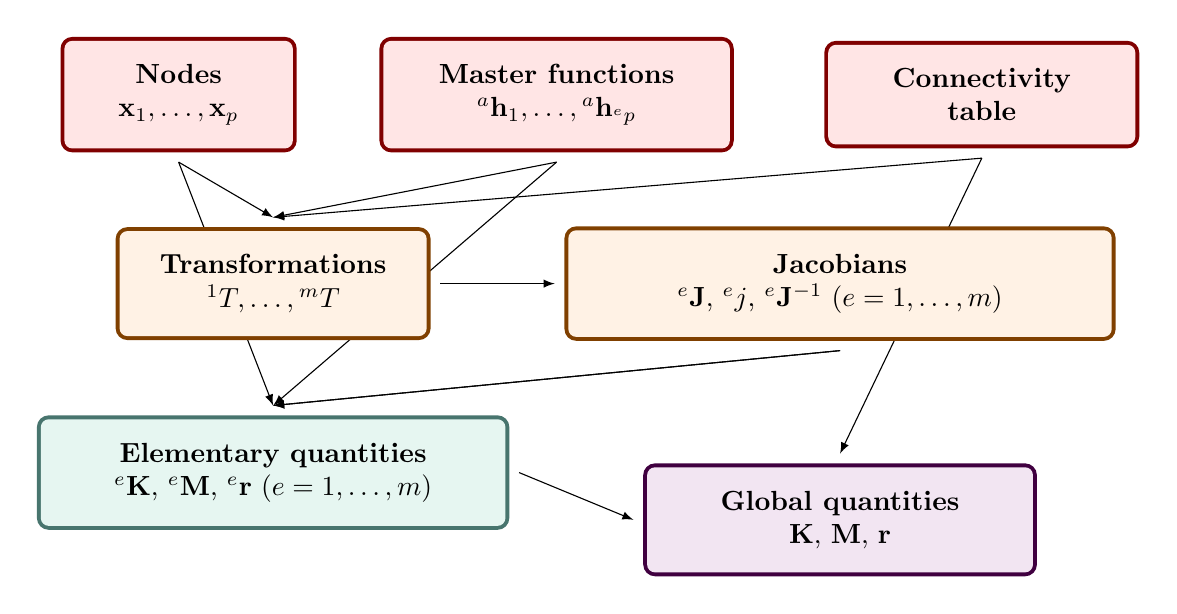
\begin{tikzpicture}[scale=0.6]
    \node (nc) at (-2,8) {
      \begin{tcolorbox}[colframe=red!50!black, colback=red!10, coltitle=black, rounded corners, width=3cm]
        \centering \textbf{Nodes} \\ $\mathbf x_1,\dots, \mathbf x_p$
      \end{tcolorbox}
    };
    \node (msf) at (6,8) {
      \begin{tcolorbox}[colframe=red!50!black, colback=red!10, coltitle=black, rounded corners,width=4.5cm]
        \centering \textbf{Master functions} \\ ${}^a \mathbf h_1,\dots,{}^a \mathbf h_{{}^ep}$
      \end{tcolorbox}
    };
    \node (ct) at (15,8) {
      \begin{tcolorbox}[colframe=red!50!black, colback=red!10, coltitle=black, rounded corners,width=4cm]
        \centering \textbf{Connectivity table}
      \end{tcolorbox}
    };
    \node (elem) at (0,0) {
      \begin{tcolorbox}[colframe=Emerald!50!black, colback=Emerald!10, coltitle=black, rounded corners,width=6cm]
        \centering \textbf{Elementary quantities} \\ ${}^e \mathbf K$, ${}^e \mathbf M$, ${}^e \mathbf r$ ($e=1,\dots, m$)
      \end{tcolorbox}
    };

    \node (glob) at (12,-1) {
      \begin{tcolorbox}[colframe=violet!50!black, colback=violet!10, coltitle=black, rounded corners,width=5cm]
        \centering \textbf{Global quantities} \\ $\mathbf K$, $\mathbf M$, $\mathbf r$
      \end{tcolorbox}
    };
    % Drawing arrows
    \draw[-latex, ] (elem.east) -- (glob.west);
    \draw[-latex, ] (msf.south) -- (elem.north);
    \draw[-latex, ] (ct.south) -- (glob.north);
    \draw[-latex, ] (nc.south) -- (elem.north);
    % Boxes
    \node (tr) at (0,4) {
      \begin{tcolorbox}[colframe=orange!50!black, colback=orange!10, coltitle=black, rounded corners,width=4cm]
        \centering \textbf{Transformations} \\ ${}^1 T,\dots,{}^{m} T$
      \end{tcolorbox}
    };

    \node (jac) at (12,4) {
      \begin{tcolorbox}[colframe=orange!50!black, colback=orange!10, coltitle=black, rounded corners,width=7cm]
        \centering \textbf{Jacobians} \\ ${}^e \mathbf J$, ${}^e j$, ${}^e \mathbf J^{-1}$ ($e=1,\dots, m$)
      \end{tcolorbox}
    };
    % Drawing arrows
    \draw[-latex, ] (nc.south) -- (tr.north);
    \draw[-latex, ] (msf.south) -- (tr.north);
    \draw[-latex, ] (ct.south) -- (tr.north);
    \draw[-latex, ] (tr.east) -- (jac.west);
    \draw[-latex, ] (jac.south) -- (elem.north);
    \draw[-latex, ] (jac.south) -- (elem.north);
  \end{tikzpicture}
\end{frame}

\begin{frame}{Isoparametric, subparametric, superparametric elements}
  \begin{block}{}
    Displacement field as well as the geometrical representation of the finite elements could be approximated using different sets of shape functions.
  \end{block}
  \begin{itemize}
    \item \textbf{Geometrical representation}
          $$
            {}^eT : \mathbf x(\boldxi)={}^a\mathbf H(\boldxi) ^e{} \mathbf x
          $$
    \item  \textbf{Displacement field approximation}
          $$
            {}^e\mathbf u^{h}(\mathbf x,t)={}^a\mathbf H(\boldxi(\mathbf x)){}^e\mathbf q(t)
          $$
  \end{itemize}
  \begin{enumerate}
    \item Subparametric: less nodes for geometric than for displacement,
    \item Isoparametric: same nodes for both geometry and displacement,
    \item Superparametric: more nodes for geometric than for displacement.
  \end{enumerate}
\end{frame}

\section{Example: modal analysis of a clamped beam}

\begin{frame}{Modal analysis of a clamped beam}
  \footnotesize\textbf{Kinematic assumptions:}
  \begin{itemize}
    \item The beam is made of elastic material which is homogeneous and isotropic ($E$, $\nu$ and $\rho$).
    \item Assume a plane stress state (very small thickness). The structure can be modeled in the $(x,y)$ plane using two-dimensional finite elements.
  \end{itemize}
  \vspace{-.3cm}
  \begin{columns}
    \column{0.65\textwidth}
    \begin{center}
      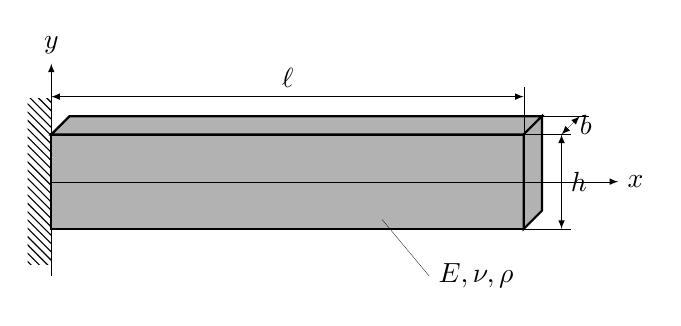
\begin{tikzpicture}[scale=0.6]
        \def\l{10}
        \def\h{2}
        \def\b{1}
        % Draw the wall 
        \fill[pattern=north west lines] (-0.5,-\h+0.25,0) rectangle (0,\h-0.25,0);
        % Draw the rectangle
        \filldraw[fill=gray!60, draw=black,thick] (0,-\h/2,0) rectangle (\l,\h/2,0);
        \draw[fill=gray!60, draw=black,thick] (0,\h/2,0) -- (0,\h/2,-\b) -- (\l,\h/2,-\b) -- (\l,\h/2,0) -- cycle;
        \draw[fill=gray!60, draw=black,thick] (\l,-\h/2,0) -- (\l,-\h/2,-\b) -- (\l,\h/2,-\b) -- (\l,\h/2,0) -- cycle;
        %axis
        \draw[-latex,ultra thin] (0,0) -- (12,0) node[right]{$x$};
        \draw[-latex, ultra thin] (0,-2) -- (0,2.5)node[above]{$y$};
        % length
        \draw[ultra thin] (\l,0) -- (\l, 2) ;
        \draw[latex-latex, ultra thin]  (0,1.8,0)  to node[midway,above] {$\ell$}(\l,1.8,0) ;
        \draw[ultra thin] (\l,\h/2) -- (\l+1, \h/2) ;
        \draw[ultra thin] (\l,-\h/2) -- (\l+1, -\h/2) ;
        \draw[latex-latex, ultra thin]  (\l+0.8,\h/2,0)  to node[midway,right] {$h$}(\l+0.8,-\h/2,0) ;
        \draw[ultra thin] (\l,\h/2,-\b) -- (\l+1, \h/2,-\b) ;
        \draw[latex-latex, ultra thin]  (\l+0.8,\h/2,0)  to node[midway,right] {$b$}(\l+0.8,\h/2,-\b) ;
        \draw[ultra thin]  (7,-0.8) -- (8,-2) node[right]{$E,\nu,\rho$};
      \end{tikzpicture}
    \end{center}

    \column{0.5\textwidth}
    {\tiny \begin{itemize}\setlength\itemsep{0.05em}
        \item $E=210\ GPa$ Young's modulus
        \item $\nu=0.3$ Poisson's ratio
        \item $\rho=7800\ kg/m^3$ material density
        \item $\ell=2\ m$ length
        \item $h=0.5\ m$ height
        \item $b=0.01\ m$ thickness
        \item $x$ axial coordinate
        \item $y$ transversal coordinate
      \end{itemize}}
  \end{columns}
  \begin{block}{Variables:}
    \begin{multicols}{2}
      \begin{itemize}\setlength\itemsep{0.05em}
        \item $u_{1}(x,y,t)$ axial displacement
        \item $u_{2}(x,y,t)$ transversal displacement\vspace{.1cm}
      \end{itemize}
    \end{multicols}
  \end{block}
\end{frame}

\begin{frame}{Modal analysis of a clamped beam}
  Discretization into $8$ bilinear quadrilateral finite elements ($4$ nodes each)
  \vspace{-0.3cm}
  \begin{center}
    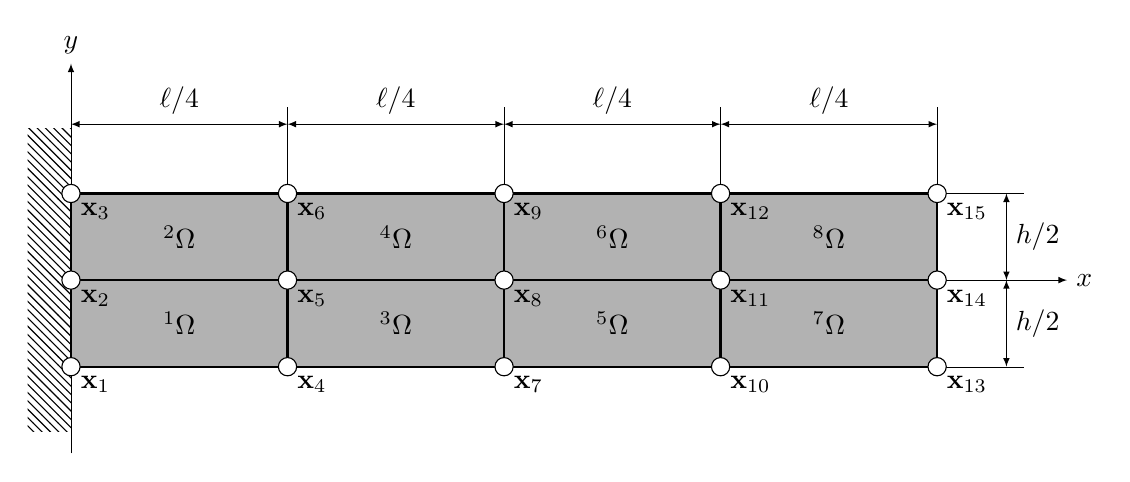
\begin{tikzpicture}[scale=1.1]
      \def\l{10}
      \def\h{2}
      \def\b{1}
      % Draw the wall 
      \fill[pattern=north west lines] (-0.5,-\h+0.25,0) rectangle (0,\h-0.25,0);
      % Draw the rectangle
      \filldraw[fill=gray!60, draw=black,thick] (0,-\h/2,0) rectangle (\l,\h/2,0);
      % Draw the elements  
      \draw[thick] (\l/4,-\h/2) -- (\l/4,\h/2);
      \draw[thick] (\l/2,-\h/2) -- (\l/2,\h/2);
      \draw[thick] (3*\l/4,-\h/2) -- (3*\l/4,\h/2);
      \draw[thick] (0,0) -- (\l,0);
      \node at (\l/8,-\h/4) {${}^1\Omega$};
      \node at (\l/8,\h/4) {${}^2\Omega$};
      \node at (\l/4+\l/8,-\h/4) {${}^3\Omega$};
      \node at (\l/4+\l/8,\h/4) {${}^4\Omega$};
      \node at (\l/2+\l/8,-\h/4) {${}^5\Omega$};
      \node at (\l/2+\l/8,\h/4) {${}^6\Omega$};
      \node at (3*\l/4+\l/8,-\h/4) {${}^7\Omega$};
      \node at (3*\l/4+\l/8,\h/4) {${}^8\Omega$};
      %axis
      \draw[-latex,ultra thin] (0,0) -- (11.5,0) node[right]{$x$};
      \draw[-latex, ultra thin] (0,-2) -- (0,2.5)node[above]{$y$};
      % length
      \draw[ultra thin] (\l/4,0) -- (\l/4, 2) ;
      \draw[ultra thin] (\l/2,0) -- (\l/2, 2) ;
      \draw[ultra thin] (3*\l/4,0) -- (3*\l/4, 2) ;
      \draw[ultra thin] (\l,0) -- (\l, 2) ;
      \draw[latex-latex, ultra thin]  (0,1.8,0)  to node[midway,above] {$\ell/4$}(\l/4,1.8,0) ;
      \draw[latex-latex, ultra thin]  (\l/4,1.8,0)  to node[midway,above] {$\ell/4$}(\l/2,1.8,0) ;
      \draw[latex-latex, ultra thin]  (\l/2,1.8,0)  to node[midway,above] {$\ell/4$}(3*\l/4,1.8,0) ;
      \draw[latex-latex, ultra thin]  (3*\l/4,1.8,0)  to node[midway,above] {$\ell/4$}(\l,1.8,0) ;
      \draw[ultra thin] (\l,-\h/2) --(\l+1, -\h/2) ;
      \draw[ultra thin] (\l,\h/2) -- (\l+1, \h/2) ;
      \draw[latex-latex, ultra thin]  (\l+0.8,\h/2,0)  to node[midway,right] {$h/2$}(\l+0.8,0,0) ;
      \draw[latex-latex, ultra thin]  (\l+0.8,-\h/2,0)  to node[midway,right] {$h/2$}(\l+0.8,0,0) ;
      % Nodes 
      \draw[fill=white, draw=black]  (0,-\h/2) node[below right]{$\mathbf x_1$} circle (3pt);
      \draw[fill=white, draw=black]  (0,0) node[below right]{$\mathbf x_2$} circle (3pt);
      \draw[fill=white, draw=black]  (0,\h/2) node[below right]{$\mathbf x_3$} circle (3pt);
      \draw[fill=white, draw=black]  (\l/4,-\h/2) node[below right]{$\mathbf x_4$} circle (3pt);
      \draw[fill=white, draw=black]  (\l/4,0) node[below right]{$\mathbf x_5$} circle (3pt);
      \draw[fill=white, draw=black]  (\l/4,\h/2) node[below right]{$\mathbf x_6$} circle (3pt);
      \draw[fill=white, draw=black]  (\l/2,-\h/2) node[below right]{$\mathbf x_7$} circle (3pt);
      \draw[fill=white, draw=black]  (\l/2,0) node[below right]{$\mathbf x_8$} circle (3pt);
      \draw[fill=white, draw=black]  (\l/2,\h/2) node[below right]{$\mathbf x_9$} circle (3pt);
      \draw[fill=white, draw=black]  (3*\l/4,-\h/2) node[below right]{$\mathbf x_{10}$} circle (3pt);
      \draw[fill=white, draw=black]  (3*\l/4,0) node[below right]{$\mathbf x_{11}$} circle (3pt);
      \draw[fill=white, draw=black]  (3*\l/4,\h/2) node[below right]{$\mathbf x_{12}$} circle (3pt);
      \draw[fill=white, draw=black]  (\l,-\h/2) node[below right]{$\mathbf x_{13}$} circle (3pt);
      \draw[fill=white, draw=black]  (\l,0) node[below right]{$\mathbf x_{14}$} circle (3pt);
      \draw[fill=white, draw=black]  (\l,\h/2) node[below right]{$\mathbf x_{15}$} circle (3pt);
    \end{tikzpicture}
  \end{center}
  \begin{block}{}
    \textbf{Objective:} determine the lower natural frequencies of the beam.
  \end{block}
  \vfill
  \begin{center}
    \href{https://drive.mathworks.com/sharing/6a9792ef-d0a7-4aca-a1d0-8b1862b0ac3b}{\beamergotobutton{Go to Matlab Drive}}
  \end{center}
  \vfill
\end{frame}

\end{document}